% Options for packages loaded elsewhere
\PassOptionsToPackage{unicode}{hyperref}
\PassOptionsToPackage{hyphens}{url}
%
\documentclass[
  letterpaper,
  DIV=11,
  numbers=noendperiod]{scrartcl}

\usepackage{amsmath,amssymb}
\usepackage{iftex}
\ifPDFTeX
  \usepackage[T1]{fontenc}
  \usepackage[utf8]{inputenc}
  \usepackage{textcomp} % provide euro and other symbols
\else % if luatex or xetex
  \usepackage{unicode-math}
  \defaultfontfeatures{Scale=MatchLowercase}
  \defaultfontfeatures[\rmfamily]{Ligatures=TeX,Scale=1}
\fi
\usepackage{lmodern}
\ifPDFTeX\else  
    % xetex/luatex font selection
\fi
% Use upquote if available, for straight quotes in verbatim environments
\IfFileExists{upquote.sty}{\usepackage{upquote}}{}
\IfFileExists{microtype.sty}{% use microtype if available
  \usepackage[]{microtype}
  \UseMicrotypeSet[protrusion]{basicmath} % disable protrusion for tt fonts
}{}
\makeatletter
\@ifundefined{KOMAClassName}{% if non-KOMA class
  \IfFileExists{parskip.sty}{%
    \usepackage{parskip}
  }{% else
    \setlength{\parindent}{0pt}
    \setlength{\parskip}{6pt plus 2pt minus 1pt}}
}{% if KOMA class
  \KOMAoptions{parskip=half}}
\makeatother
\usepackage{xcolor}
\setlength{\emergencystretch}{3em} % prevent overfull lines
\setcounter{secnumdepth}{5}
% Make \paragraph and \subparagraph free-standing
\makeatletter
\ifx\paragraph\undefined\else
  \let\oldparagraph\paragraph
  \renewcommand{\paragraph}{
    \@ifstar
      \xxxParagraphStar
      \xxxParagraphNoStar
  }
  \newcommand{\xxxParagraphStar}[1]{\oldparagraph*{#1}\mbox{}}
  \newcommand{\xxxParagraphNoStar}[1]{\oldparagraph{#1}\mbox{}}
\fi
\ifx\subparagraph\undefined\else
  \let\oldsubparagraph\subparagraph
  \renewcommand{\subparagraph}{
    \@ifstar
      \xxxSubParagraphStar
      \xxxSubParagraphNoStar
  }
  \newcommand{\xxxSubParagraphStar}[1]{\oldsubparagraph*{#1}\mbox{}}
  \newcommand{\xxxSubParagraphNoStar}[1]{\oldsubparagraph{#1}\mbox{}}
\fi
\makeatother


\providecommand{\tightlist}{%
  \setlength{\itemsep}{0pt}\setlength{\parskip}{0pt}}\usepackage{longtable,booktabs,array}
\usepackage{calc} % for calculating minipage widths
% Correct order of tables after \paragraph or \subparagraph
\usepackage{etoolbox}
\makeatletter
\patchcmd\longtable{\par}{\if@noskipsec\mbox{}\fi\par}{}{}
\makeatother
% Allow footnotes in longtable head/foot
\IfFileExists{footnotehyper.sty}{\usepackage{footnotehyper}}{\usepackage{footnote}}
\makesavenoteenv{longtable}
\usepackage{graphicx}
\makeatletter
\def\maxwidth{\ifdim\Gin@nat@width>\linewidth\linewidth\else\Gin@nat@width\fi}
\def\maxheight{\ifdim\Gin@nat@height>\textheight\textheight\else\Gin@nat@height\fi}
\makeatother
% Scale images if necessary, so that they will not overflow the page
% margins by default, and it is still possible to overwrite the defaults
% using explicit options in \includegraphics[width, height, ...]{}
\setkeys{Gin}{width=\maxwidth,height=\maxheight,keepaspectratio}
% Set default figure placement to htbp
\makeatletter
\def\fps@figure{htbp}
\makeatother
% definitions for citeproc citations
\NewDocumentCommand\citeproctext{}{}
\NewDocumentCommand\citeproc{mm}{%
  \begingroup\def\citeproctext{#2}\cite{#1}\endgroup}
\makeatletter
 % allow citations to break across lines
 \let\@cite@ofmt\@firstofone
 % avoid brackets around text for \cite:
 \def\@biblabel#1{}
 \def\@cite#1#2{{#1\if@tempswa , #2\fi}}
\makeatother
\newlength{\cslhangindent}
\setlength{\cslhangindent}{1.5em}
\newlength{\csllabelwidth}
\setlength{\csllabelwidth}{3em}
\newenvironment{CSLReferences}[2] % #1 hanging-indent, #2 entry-spacing
 {\begin{list}{}{%
  \setlength{\itemindent}{0pt}
  \setlength{\leftmargin}{0pt}
  \setlength{\parsep}{0pt}
  % turn on hanging indent if param 1 is 1
  \ifodd #1
   \setlength{\leftmargin}{\cslhangindent}
   \setlength{\itemindent}{-1\cslhangindent}
  \fi
  % set entry spacing
  \setlength{\itemsep}{#2\baselineskip}}}
 {\end{list}}
\usepackage{calc}
\newcommand{\CSLBlock}[1]{\hfill\break\parbox[t]{\linewidth}{\strut\ignorespaces#1\strut}}
\newcommand{\CSLLeftMargin}[1]{\parbox[t]{\csllabelwidth}{\strut#1\strut}}
\newcommand{\CSLRightInline}[1]{\parbox[t]{\linewidth - \csllabelwidth}{\strut#1\strut}}
\newcommand{\CSLIndent}[1]{\hspace{\cslhangindent}#1}

\usepackage{booktabs}
\usepackage{caption}
\usepackage{longtable}
\usepackage{colortbl}
\usepackage{array}
\usepackage{anyfontsize}
\usepackage{multirow}
\KOMAoption{captions}{tableheading}
\usepackage[left]{lineno}
\linenumbers
\usepackage{xcolor}
\usepackage{float}
\floatplacement{table}{H}
\usepackage{setspace}
\makeatletter
\@ifpackageloaded{caption}{}{\usepackage{caption}}
\AtBeginDocument{%
\ifdefined\contentsname
  \renewcommand*\contentsname{Table of contents}
\else
  \newcommand\contentsname{Table of contents}
\fi
\ifdefined\listfigurename
  \renewcommand*\listfigurename{List of Figures}
\else
  \newcommand\listfigurename{List of Figures}
\fi
\ifdefined\listtablename
  \renewcommand*\listtablename{List of Tables}
\else
  \newcommand\listtablename{List of Tables}
\fi
\ifdefined\figurename
  \renewcommand*\figurename{Figure}
\else
  \newcommand\figurename{Figure}
\fi
\ifdefined\tablename
  \renewcommand*\tablename{Table}
\else
  \newcommand\tablename{Table}
\fi
}
\@ifpackageloaded{float}{}{\usepackage{float}}
\floatstyle{ruled}
\@ifundefined{c@chapter}{\newfloat{codelisting}{h}{lop}}{\newfloat{codelisting}{h}{lop}[chapter]}
\floatname{codelisting}{Listing}
\newcommand*\listoflistings{\listof{codelisting}{List of Listings}}
\makeatother
\makeatletter
\makeatother
\makeatletter
\@ifpackageloaded{caption}{}{\usepackage{caption}}
\@ifpackageloaded{subcaption}{}{\usepackage{subcaption}}
\makeatother

\ifLuaTeX
  \usepackage{selnolig}  % disable illegal ligatures
\fi
\usepackage{bookmark}

\IfFileExists{xurl.sty}{\usepackage{xurl}}{} % add URL line breaks if available
\urlstyle{same} % disable monospaced font for URLs
\hypersetup{
  pdftitle={Snow Interception Relationships with Meteorology and Canopy Structure in a Subalpine Forest},
  hidelinks,
  pdfcreator={LaTeX via pandoc}}


\title{Snow Interception Relationships with Meteorology and Canopy
Structure in a Subalpine Forest}
\author{}
\date{}

\begin{document}
\maketitle


\setstretch{1.5}

\textbf{Authors:}

A. Cebulski\textsuperscript{1} (ORCID ID - 0000-0001-7910-5056)

J.W. Pomeroy\textsuperscript{1} (ORCID ID - 0000-0002-4782-7457)

\textsuperscript{1}Centre for Hydrology, University of Saskatchewan,
Canmore, Canada

\textbf{Corresponding Author:} A. Cebulski, alexcebulski@gmail.com

\textbf{Abstract:} Snow accumulation models differ in how snow
interception and ablation processes are represented and thus their
application to diverse climates and forest types is uncertain. Existing
parameterizations of initial snow interception before unloading include
inherently coupled canopy snow accumulation and ablation processes. This
leads to difficulty in diagnosing processes and adding possible errors
to simulations when incorporated as canopy interception routines in
models that already account for canopy snow ablation. This study
evaluates the theory underpinning parameterizations of initial snow
interception using high-temporal resolution and fine-scale measurements
of throughfall for events with minimal snow ablation and redistribution
in both the canopy and on the ground. The relationship between these
throughfall measurements, event meteorology, and a novel lidar-based
canopy strucutre measurement are assessed in two subalpine forest plots
in the Canadian Rockies. Contrary to existing theories, no association
of canopy snow load or air temperature with interception efficiency was
observed. Instead, canopy structure emerged as the primary factor
governing snow accumulation. A wind-driven snowfall event demonstrated
that non-vertical hydrometeor trajectories can significantly increase
snow-leaf contact area, thereby enhancing initial interception before
ablation. Prediction of interception efficiency for this event improved
dramatically when adjusted for hydrometeor trajectory angle based on a
wind speed at one-third of the canopy height. Snow-leaf contact area
showed a high sensitivity to wind speed, increasing by up to 95\% with a
1 m s\textsuperscript{-1} wind speed. The study proposes a new
parameterization that calculates throughfall, independent of processes
that ablate snow from the canopy, as a function of snow-leaf contact
area adjusted for hydrometeor trajectory angle. This new
parameterization successfully estimated subcanopy snow accumulation for
a snowfall event at two forest plots measured using lidar and snow
surveys. By separating canopy snow ablation from snow interception
processes, this new model offers potentially improved prediction of
subcanopy snow accumulation when combined with canopy snow ablation
parameterizations.

\textbf{Keywords:} snow interception, throughfall, ablation, forest,
snowpack, lidar, process-based modelling

\section{Introduction}\label{introduction}

Over half of North America's snow-covered zone is covered by forests
(Kim et al., 2017), significantly impacting the accumulation and
redistribution of snowpacks and subsequent snowmelt runoff. Essery et
al. (2003) estimated that 25--45\% of annual snowfall may be lost to the
atmosphere due to sublimation of snow intercepted in forest canopies
globally. Snow intercepted in the canopy can sublimate and melt at much
higher rates than the subcanopy snowpack (Floyd, 2012; Lundberg \&
Hallidin, 1994; Pomeroy et al., 1998), reducing the amount of snow
available for runoff. Vegetation structure is one of the primary factors
controlling the partitioning of snowfall into throughfall and
interception, and thus governs the quantity of snow subject to
sublimation from the canopy (Hedstrom \& Pomeroy, 1998; Storck et al.,
2002). However, forest thinning efforts aimed at limiting sublimation
losses to increase snowmelt runoff do not always lead to a corresponding
increase in spring streamflow (Golding \& Swanson, 1978; Harpold et al.,
2020; Pomeroy et al., 2012; Troendle, 1983). This may be due to
increased ablation rates when forest cover is reduced, desynchronization
of snowmelt, and sub-surface hydrology interactions (Ellis et al., 2013;
Musselman et al., 2015; Pomeroy et al., 1997; Safa et al., 2021; Varhola
et al., 2010). Due to the significant impact of forest cover on snow
accumulation and ablation, and sparse or absent monitoring networks for
subcanopy snow accumulation (Rittger et al., 2020; Vionnet et al.,
2021), land management, ecological conservation and water resource
decisions rely on robust models of snow redistribution to estimate past,
current and future subcanopy snowpacks.

Hedstrom \& Pomeroy (1998), working in the cold continental boreal
forest, proposed that initial snow interception efficiency was
controlled by the maximum canopy load which itself was a function of
leaf area index and new snow density. Unloading was found to be an
exponential function of time and observed only days or weeks after the
interception event. Storck et al. (2002), working in temperate coastal
forests, emphasized the role of leaf area index and air temperature in
controlling the maximum canopy snow load. The opposing relationship
between air temperature and maximum canopy snow load in the Hedstrom \&
Pomeroy (1998) and Storck et al. (2002) parameterizations is shown in
Clark et al. (2015) Figure 4. Gelfan et al. (2004) demonstrated accurate
subcanopy snowpack simulations at study sites in Russia by treating the
Hedstrom \& Pomeroy (1998) and Storck et al. (2002) parameterizations
separately while using a step-based function to choose either
parameterization based on temperature. A similar parameterization in the
Cold Regions Hydrological Model (Pomeroy et al., 2022) has shown strong
performance at sites across Canada, northern United States, Switzerland,
and Spain. However, overestimation of subcanopy snow accumulation was
reported by Lundquist et al. (2021) and Lumbrazo et al. (2022) when
combining the Hedstrom \& Pomeroy (1998) routine with ablation
parameterizations from different studies (e.g., Roesch et al., 2001).
The coupling of ablation processes within existing snow interception
models (Hedstrom \& Pomeroy, 1998; Storck et al., 2002) may contribute
to overestimates of throughfall, canopy snow unloading, and canopy snow
melt when combined with other canopy snow ablation parameterizations
(Cebulski \& Pomeroy, 2024). Additional observations of snow
interception that exclude ablation processes could help determine the
applicability of the interception theories proposed by Hedstrom \&
Pomeroy (1998) and Storck et al. (2002). Hedstrom \& Pomeroy's (1998)
theory also suggests that moderate wind speeds, which can result in more
horizontal hydrometeor trajectories and increase the snow-leaf contact
area and interception efficiency at the plot scale. This association has
also been shown in rainfall interception studies to decrease throughfall
of rain (Herwitz \& Slye, 1995; Van Stan et al., 2011). Despite this
importance for rainfall, the relationship proposed by Hedstrom \&
Pomeroy (1998), has typically not been included in snow accumulation
models (Clark et al., 2020; Mahat \& Tarboton, 2014) as empirical
testing of this relationship is lacking.

The objective of this paper is to evaluate the theories underlying
existing snow interception models using high spatial and temporal
resolution measurements of subcanopy snow accumulation for events with
minimal canopy snow ablation. These new observations are investigated to
address the following research questions:

\begin{enumerate}
\def\labelenumi{\arabic{enumi}.}
\item
  Are the existing theories regarding the relationships between
  meteorology and forest structure and snow interception supported by
  in-situ observations?
\item
  Is snow interception influenced by non-vertical hydrometeor trajectory
  angles over a wind-driven snowfall event?
\item
  To what extent can these findings inform the development of a new
  parameterization for snow interception?
\end{enumerate}

\section{Theory}\label{theory}

\subsection{Snow interception}\label{snow-interception}

The canopy snow load, \(L\) (kg m\textsuperscript{-2}) can be estimated
from the mass balance:

\begin{equation}\phantomsection\label{eq-canopy-mass-bal}{
\frac{dL}{dt} = 
q_{sf} + q_{ros} - q_{tf} - q_{unld} - q_{drip} - q_{wind}^{veg} - q_{sub}^{veg}
}\end{equation}

where \(q_{sf}\) is the snowfall rate (kg m\textsuperscript{-2}
s\textsuperscript{-1}), \(q_{ros}\) (kg m\textsuperscript{-2}
s\textsuperscript{-1}) is the rate of rainfall falling on snow
intercepted in the canopy, \(q_{tf}\) (kg m\textsuperscript{-2}
s\textsuperscript{-1}) is the throughfall rate (kg m\textsuperscript{-2}
s\textsuperscript{-1}), \(q_{unld}\) is the canopy snow unloading rate
(kg m\textsuperscript{-2} s\textsuperscript{-1}), \(q_{drip}\) is the
canopy snow drip rate due to canopy snowmelt (kg m\textsuperscript{-2}
s\textsuperscript{-1}), \(q_{wind}^{veg}\) is the wind transport rate in
or out of the control volume (kg m\textsuperscript{-2}
s\textsuperscript{-1}), and \(q_{sub}^{veg}\) is the intercepted snow
sublimation rate (kg m\textsuperscript{-2} s\textsuperscript{-1}).
Figure 1 in Cebulski \& Pomeroy (2024) presents a visual representation
of this mass balance.

During periods with low air temperatures and low wind speeds,
\(q_{unld}\), \(q_{drip}\), \(q_{wind}^{veg}\), and \(q_{sub}^{veg}\)
can be assumed negligible. Interception efficiency, \(\frac{I}{P}\) (-),
which is the fraction of snowfall intercepted over \(\Delta t\) before
ablation, can then be calculated during these periods as:

\begin{equation}\phantomsection\label{eq-ip}{
\frac{I}{P} = \frac{\Delta L}{\overline{q_{sf}} \Delta t}
}\end{equation}

and throughfall, \(q_{tf}\) can be calculated as:

\begin{equation}\phantomsection\label{eq-event-tf}{
q_{tf} = \left(1 - \frac{I}{P} \right) \cdot q_{sf}
}\end{equation}

\subsection{Hydrometeor trajectory
angle}\label{hydrometeor-trajectory-angle}

The trajectory angle, \(\theta_h\) of a hydrometeor as the departure in
degrees (°) from a vertical plane, is shown in Herwitz \& Slye (1995) to
be calculated as:

\begin{equation}\phantomsection\label{eq-ta}{
\theta_h = \arctan \left(\frac{x_h(u_z)}{v_h(D_h)}\right)*\frac{180}{\pi}
}\end{equation}

where \(v_h(D_h)\) is the terminal fall velocity of the hydrometeor (m
s\textsuperscript{-1}), which is a function of the hydrometeor diameter,
\(D_h\) and \(x_h(u_z)\) is the horizontal velocity of the hydrometeor
(m s\textsuperscript{-1}) which is a function of the within canopy wind
speed, \(u_z\) at height above ground, \(z\). This assumes the
hydrometeors are following fluid points in the atmosphere.

\section{Data and methods}\label{data-and-methods}

\subsection{Study site}\label{study-site}

This study was conducted at Fortress Mountain Research Basin (FMRB),
Alberta, Canada, -115° W, 51° N, a continental headwater basin in the
Canadian Rockies (Figure~\ref{fig-site-map}). Data from this study was
collected between October 2021 and July 2023 within and surrounding two
forest plots adjacent to the FMRB Powerline Station (PWL) and Forest
Tower Station (FT) at \textasciitilde2100 m above sea level as shown in
Figure~\ref{fig-site-map}. The average annual precipitation at PWL
Station from 2013 to 2023 was 1045 mm, with the peak annual snow water
equivalent (SWE) reaching 465 kg m\textsuperscript{-2}, typically
occurring in late April. The PWL and FT forest plots include
discontinuous stands of 70\% subalpine fir (Abies lasiocarpa) and 30\%
Engelmann spruce (Picea engelmannii) (Langs et al., 2020). The PWL plot
is located 120 m to the northwest of FT station and contains a forest
clearing with a diameter of \textasciitilde12 m, surrounded by a closed
canopy. The canopy coverages of the two forest plots are 0.51 and 0.29
and the winter leaf area indices are 2.07 and 1.66 for PWL and FT
respectively. The average height of the canopy surrounding the plot to
the east of the PWL station is 10.5 m and surrounding the forest plot
around the FT Station is 7.1 m. The forest of the FT plot has a
discontinuous canopy without artificial clearings. In August of 1936,
the majority of vegetation in FMRB burned during a large forest fire
that affected most of the Kananaskis Valley (Fryer et al., 1988).
Following the fire, the forest within the PWL and FT forest plots has
naturally regenerated, though some trees have been removed for road
clearing and creation of a snow study plot.

\begin{figure}[H]

\centering{

\includegraphics{figs/maps/site_map_inset.png}

}

\caption{\label{fig-site-map}Map showing the location of forest plots,
flux towers, subcanopy lysimeter instruments (SCL), and survey
transects. The inset map on the lower right shows the regional location
of Fortress Mountain Research basin.}

\end{figure}%

\subsection{Meteorological
measurements}\label{meteorological-measurements}

Measurements of air temperature and relative humidity (Vaisala model
HMP155A), wind speed and direction (RM Young model 86000 2-D ultrasonic
anemometer) were made 4.3 m above the ground at FT station
(Figure~\ref{fig-site-map}). Wind speed measurements from a 3-cup
anemometer (Met One model 014A), installed adjacent to the 2-D
ultrasonic anemometer at 4.3 m, were used for gap filling wind speed.
Additional wind speed measurements were collected by two 3D sonic
anemometers (Campbell Scientific CSAT3) installed at 2 m (raised to 3 m
February 2022) and 13.5 m above the ground at FT station. Average wind
speeds at these four heights were found to follow a logarithmic
relationship for periods where the instruments were known to be clean of
snow. Thus, a wind profile was fitted to these measurements using the
Prandtl-von Kármán log-linear relationship:

\begin{equation}\phantomsection\label{eq-log-wind-profile}{
\overline{u} = \frac{u_*}{k} ln(\frac{z - d_0}{z_0})
}\end{equation}

where \(\overline{u}\) is average wind speed (m s\textsuperscript{-1})
at height, \(z\) (m) above the ground, \(u_*\) is the friction velocity
(m s\textsuperscript{-1}), \(d_0\) is the displacement height (m),
\(z_0\) is the roughness length of momentum (m), and \(k\) is the
dimensionless von Kármán Constant (0.4).

To determine the displacement height and roughness length parameters the
function ``optim'' from the stats R package (R Core Team, 2024) was
used. The parameters found for the wind speed profile include a
roughness length of 0.50 m and displacement height of 0.58 m. See the
supporting information for more information on the development and
testing of the wind profile. At PWL station, the snowfall rate was
measured by an Alter-shielded OTT Pluvio weighing precipitation gauge
2.6 m above ground, corrected for undercatch following phase correction
by Harder \& Pomeroy (2013) and catch efficiency by Smith (2007). Wind
speed for undercatch correction was measured by a 3-cup anemometer (Met
One model 014A) at a height of 2.6 m at PWL station. An optical
disdrometer (OTT Parsivel2) provided measurements of hydrometeor
particle size and vertical velocity. All measurements were recorded at
15-min intervals using Campbell Scientific dataloggers, except the
Parsivel2 which was recorded at 1-minute intervals by an onsite
computer.

\subsection{Lysimeter measurements}\label{lysimeter-measurements}

Three subcanopy lysimeters (SCLs) were installed surrounding the FT
Station (Figure~\ref{fig-site-map}) to provide 15-minute interval
measurements of throughfall as in MacDonald (2010).
Figure~\ref{fig-scl-imgs} shows the three SCLs which consisted of a
plastic horse-watering trough with an opening of 0.9
m\textsuperscript{2} and depth of 20 cm suspended from a load cell
(Intertechnology 9363-D3-75-20T1) attached to an aluminum pipe connected
between two trees. For 26 distinct snowfall events, where canopy snow
ablation rates were deemed negligible, the throughfall rate, \(q_{tf}\),
was calculated by dividing the weight of snow in the SCL by the
cross-sectional area of the SCL opening and determining the rate of
change at 15-minute intervals. Canopy snow load was estimated at the
same 15-minute intervals during these events using
Equation~\ref{eq-canopy-mass-bal} and incorporating measurements of
\(q_{tf}\) from the SCLs and \(q_{sf}\) from the PWL snowfall gauge.
Interception efficiency was also calculated for these intervals using
Equation~\ref{eq-ip}. Timelapse imagery, mass change on a weighed tree
lysimeter ``hanging tree'' (Pomeroy \& Schmidt, 1993) and in-situ
observations were used to ensure the ablation of snow intercepted in the
canopy was minimal over each interval. Additionally, the \(q_{tf}\)
measurements were filtered to include observations with a snowfall rate
\textgreater{} 0 kg m\textsuperscript{-2} hr\textsuperscript{-1},
throughfall rate \textgreater{} 0.05 kg m\textsuperscript{-2}
hr\textsuperscript{-1} and a snowfall rate greater than the subcanopy
lysimeter throughfall rate to minimize observations with unloading. The
weighed tree lysimeter, a live subalpine fir (Abies lasiocarpa) tree
suspended from a load cell (Artech S-Type 20210-100) measured the weight
of canopy snow load, \(L_{wt}\) (kg). The weight of snow intercepted on
the weighed tree was scaled to an areal estimate of canopy snow load
(\(L\), kg m\textsuperscript{-2}) using measurements of areal
throughfall (kg m\textsuperscript{-2}) from manual snow surveys and
snowfall from the PWL Station snowfall gauge (see description of method
in Pomeroy \& Schmidt, 1993). The canopy structure surrounding three
SCLs is shown in Figure~\ref{fig-scl-imgs} and was measured using
hemispherical photography (Nikon Coolpix 4500 and EC-F8 hemispherical
lens) and the hemispheR R package Chianucci \& Macek (2023). The leaf
area index and canopy coverage from hemispherical photo analysis is
shown in Table~\ref{tbl-scl-lai-cc}.

\begin{longtable}[]{@{}lrr@{}}

\caption{\label{tbl-scl-lai-cc}Canopy structure of the three subcanopy
lysimeters (SCL) located proximal to the FT Station. Leaf area index
(LAI) and Canopy Coverage was measured using hemispherical photo
analysis with the R package hemispheR.}

\tabularnewline

\toprule\noalign{}
Name & LAI (-) & Canopy Coverage (-) \\
\midrule\noalign{}
\endhead
\bottomrule\noalign{}
\endlastfoot
Sparse & 1.59 & 0.73 \\
Mixed & 1.86 & 0.78 \\
Closed & 2.11 & 0.82 \\

\end{longtable}

\begin{figure}[H]

\centering{

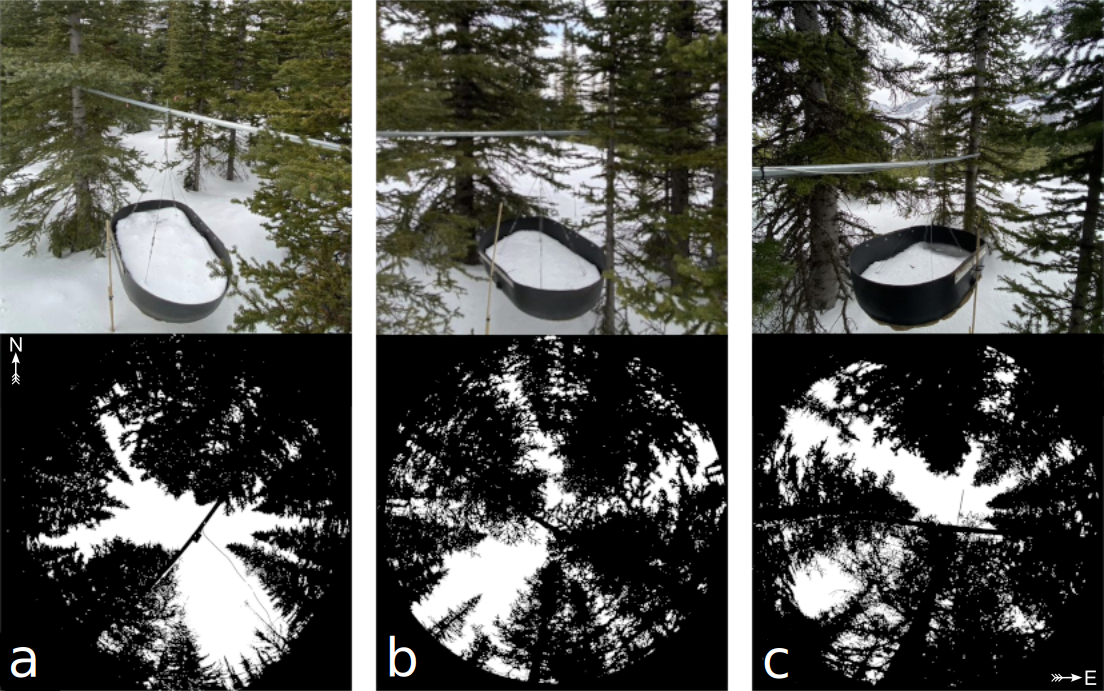
\includegraphics{figs/site-photos/scl_w_fisheye_textnew.png}

}

\caption{\label{fig-scl-imgs}Images of the three subcanopy lysimeters
(SCL) and surrounding canopy located in sparse (a), mixed (b), and dense
(c) canopy. The top row presents a side view of each SCL and the bottom
row shows hemispherical photographs classified using the hemispheR R
package. These hemispherical images are oriented with north at the top
and have been flipped to provide a view from above (i.e., east is on the
right side of each image).}

\end{figure}%

\subsection{UAV-Lidar data cCollection and
processing}\label{uav-lidar-data-ccollection-and-processing}

The UAV (FreeFly Alta X) payload included a REIGL miniVUX-2 airborne
laser scanner, an Applanix APX-20 inertial measurement unit (IMU) and
global navigation satellite system (GNSS). The UAV was flown 90 m above
the ground at a speed of 3 m s\textsuperscript{-1} following the path
shown in Figure~\ref{fig-site-map}. A detailed description of the UAV,
payload, and flight settings is provided in the supporting information.
The methods outlined by Harder et al. (2020) and Staines \& Pomeroy
(2023) were incorporated to reconcile survey lidar, IMU and GNSS data. A
vertical offset of up to 6 cm between UAV-lidar flight lines was
observed in the resulting point clouds on March 13\textsuperscript{th}
and 14\textsuperscript{th}, 2024 and was attributed to IMU position
drift. This offset between flight lines was corrected using the
BayesStripAlign software v2.24 (BayesMap Solutions, 2024). After strip
alignment, the mean elevation bias was 0.000 m and the RMS error
declined from 0.055 m to 0.038 m on March 13\textsuperscript{th} and
changed from 0.033 m to 0.029 m on March 14\textsuperscript{th}. The
point cloud density ranged from \textasciitilde1200 returns
m\textsuperscript{2} in sparse forest to \textasciitilde2200 returns
m\textsuperscript{2} in open clearings after flight paths were combined
for each survey. Quality control, ground classification, calculation of
the change in between two UAV-lidar point clouds, and raster generation
(0.05 m grid cell resolution) was conducted using the LAStools software
package (LAStools, 2024). Post processing and resampling of raster data
to a 0.25 m grid cell resolution was conducted using the `Terra' R
package (Hijmans, 2024). More details on the UAV-lidar processing
workflow are provided in the supporting information.

\subsection{Snow surveys}\label{snow-surveys}

\subsubsection{In-situ snow depth and
density}\label{in-situ-snow-depth-and-density}

Twelve in-situ fresh snow surveys (six pre- and post-snowfall event
pairs) provided measurements of subcanopy throughfall depth and density
at 30 locations following the transects shown in
Figure~\ref{fig-site-map} to upscale the weighed tree snow load as in
Hedstrom \& Pomeroy (1998). Minimal ablation and redistribution of snow
was observed between the pre- and post-snowfall surveys. When conditions
allowed for a UAV-lidar flight, the in-situ snow surveys were conducted
following the UAV-lidar flight to assess the accuracy of the throughfall
measurements and provide a fresh snow density for the calculation of SWE
(kg m\textsuperscript{-2}). A 1000 cm\textsuperscript{3} Perla snow
density wedge sampler (RIP Cutter,
https://snowmetrics.com/shop/rip-1-cutter-1000-cc/) was used to measure
the density of the fresh snow layer, \(\overline{\rho_{tf}}\) (kg
m\textsuperscript{-3}) from snow pits. Throughfall depth measurements,
\(\Delta HS\) were converted to SWE using the following equation:

\begin{equation}\phantomsection\label{eq-swe-tf}{
\Delta SWE_{tf} = \Delta HS \cdot \overline{\rho_{tf}}
}\end{equation}

Differential GNSS rover coordinates, with ± 2.5 cm 3D uncertainty, were
taken at each snow sampling location so the locations could be queried
later from the UAV-lidar rasters to assess measurement error and were
also used as input for the UAV-lidar strip alignment. If a pre-event
crust layer was present, the depth of post event fresh snow accumulation
above the crust layer was interpreted as throughfall over the event. In
the absence of a defined crust layer, the difference in pre- and
post-event snow depth to ground was interpreted as event throughfall.

\subsubsection{UAV-Lidar snow depth}\label{uav-lidar-snow-depth}

Two uncrewed aerial vehicle (UAV) lidar surveys were conducted before
and after a 24-hour snowfall event that occurred between March
13\textsuperscript{th} and March 14\textsuperscript{th}, 2023 to
facilitate the measurement of snow accumulation and canopy structure
within the FT and PWL forest plots. This period was selected based on
two criteria: 1) it provided sufficient cumulative snowfall to result in
a low relative error in UAV-LiDAR measured throughfall, and (2) minimal
redistribution and ablation was observed, as confirmed by the SCLs,
weighed tree, and time-lapse imagery. The change in elevation between
the two UAV-lidar surveys was interpreted as the increase in snow
accumulation, \(\Delta HS\) over the snowfall event.

\subsection{UAV-Lidar canopy metrics}\label{uav-lidar-canopy-metrics}

To characterize the canopy structure, the voxel ray sampling (VoxRS)
methodology for lidar data analysis was employed, as developed by
Staines \& Pomeroy (2023), for the two UAV-lidar surveys. This method
was chosen for its ability to provide canopy metrics that are less
sensitive to the inherent non-uniform nature of lidar sampling data,
which often results from beam occlusion in vegetation and leads to
reduced points near the ground. Using this method radiation
transmittance, \(\tau\) (-), was measured across the hemisphere at a 1°
step, i.e., azimuth angles (0°, 1°, \ldots, 359°) and zenith angles (0°,
1°, \ldots, 90°) for each 0.25 m grid cell within the FT and PWL forest
plots. The fraction of snow-leaf contact area per unit area of ground
proposed by Hedstrom \& Pomeroy (1998), and hereafter called leaf
contact area (\(C_p\)), was then calculated as:

\begin{equation}\phantomsection\label{eq-lca}{
C_p(C_c, \theta_h, L) = 1-\tau
}\end{equation}

\begin{equation}\phantomsection\label{eq-tf-ode}{
C_p(C_c, \theta_h, L) = \begin{cases}
    1-\tau,& \text{if } \theta_h> 0°\\
    1-\tau \approx C_c ,              & \theta_h= 0°
\end{cases}
}\end{equation}

where \(C_p\) is a function of the canopy coverage \(C_c\), \(\theta_h\)
and \(L\). \(C_p\) is approximately equal to canopy coverage (\(C_c\))
for vertical snowfall trajectories. However, for non-vertical snowfall
\(1 > C_p > C_c\).

\subsection{Statistics and regression
models}\label{statistics-and-regression-models}

To determine how forest structure was associated with interception
efficiency at different azimuth and zenith angles over the March 13---14
snowfall event, the entire hemisphere at each grid location was
considered. The relationship between interception efficiency and canopy
contact number was found to be linear and thus the Pearson Correlation
Coefficient, \(\rho_p\) was calculated using the `stats' package in R (R
Core Team, 2024) to quantify the association between a single raster of
interception efficiency and the 32,760 rasters containing the canopy
contact number hemisphere for each portion of the hemisphere (azimuth
{[}0°, 1°, \ldots, 359°{]}, zenith angle {[}0°, 1°, \ldots, 90°{]}) for
each of the 25 cm grid cells across the FT and PWL forest plots.

Linear and non-linear regression models were developed to assess
relationships in the observed data. Linear models were fitted using
ordinary least squares regression via the `lm' function from the R
`stats' package (R Core Team, 2024) to analyze two relationships: (1)
between interception efficiency and meteorological variables and (2)
between interception efficiency and leaf contact area. The latter was
forced through the origin based on the theoretical justification that
the dependent variable should be zero when the independent variable is
zero. Kozak \& Kozak (1995) noted, the default
\emph{R}\textsuperscript{2} value provided for least squares models
forced through the origin by many statistical packages can be
misleading. Therefore, these \emph{R}\textsuperscript{2} values were
adjusted using Equation 10 in Kozak \& Kozak (1995). Non-linear models
were fitted using non-linear least squares regression via the `nls'
function in `stats' package in R.

\section{Results}\label{results}

\subsection{The influence of meteorology on snow
interception}\label{the-influence-of-meteorology-on-snow-interception}

Canopy snow load was estimated for 26 snowfall events and increased
linearly with cumulative event snowfall without evidence of reaching a
maximum (Figure~\ref{fig-scl-w-sf}). Over these events, air temperature
ranged from -24.5°C to 1°C, wind speeds at 4.3 m height ranged from calm
to 4.6 m s\textsuperscript{-1} (Table~\ref{tbl-sf-event-met}), and wind
direction was predominately from the southwest during snowfall
(Figure~\ref{fig-wind-rose}). Missing canopy snow load measurements in
Figure~\ref{fig-scl-w-sf} for certain troughs during specific events was
caused by damage to the subcanopy lysimeter wiring due to animals and
heavy snow loads.

\begin{figure}[H]

\centering{

\includegraphics{figs/automated_snowfall_event_periods/cuml_event_snowfall_canopy_storage_sep_scl.png}

}

\caption{\label{fig-scl-w-sf}Plot showing the cumulative event snowfall
versus the corresponding state of canopy snow load calculated using the
SCLs for each of the 26 snowfall events. The SCLs are denoted by a
distinct colour (grey, yellow, and green), correspond to varying canopy
coverage (0.73, 0.78, and 0.82, respectively).}

\end{figure}%

\pagebreak
\setstretch{1.0}

\begin{table}

\caption{\label{tbl-sf-event-met}Meteorology of the 26 snowfall events.
Air temperature and wind speed were measured at FT station. Snowfall was
measured at PWL station. Interception efficiency is estimated from
snowfall and the average throughfall of all three SCLs located within
the FT forest plot (all from 15-min. measurements).}

\centering{

\fontsize{12.0pt}{14.4pt}\selectfont
\begin{tabular*}{\linewidth}{@{\extracolsep{\fill}}>{\centering\arraybackslash}p{\dimexpr 67.50pt -2\tabcolsep-1.5\arrayrulewidth}>{\centering\arraybackslash}p{\dimexpr 37.50pt -2\tabcolsep-1.5\arrayrulewidth}>{\centering\arraybackslash}p{\dimexpr 37.50pt -2\tabcolsep-1.5\arrayrulewidth}>{\centering\arraybackslash}p{\dimexpr 37.50pt -2\tabcolsep-1.5\arrayrulewidth}>{\centering\arraybackslash}p{\dimexpr 37.50pt -2\tabcolsep-1.5\arrayrulewidth}>{\centering\arraybackslash}p{\dimexpr 37.50pt -2\tabcolsep-1.5\arrayrulewidth}>{\centering\arraybackslash}p{\dimexpr 37.50pt -2\tabcolsep-1.5\arrayrulewidth}>{\centering\arraybackslash}p{\dimexpr 37.50pt -2\tabcolsep-1.5\arrayrulewidth}>{\centering\arraybackslash}p{\dimexpr 37.50pt -2\tabcolsep-1.5\arrayrulewidth}>{\centering\arraybackslash}p{\dimexpr 37.50pt -2\tabcolsep-1.5\arrayrulewidth}>{\centering\arraybackslash}p{\dimexpr 60.00pt -2\tabcolsep-1.5\arrayrulewidth}}
\toprule
 & \multicolumn{3}{>{\centering\arraybackslash}m{\dimexpr 112.50pt -2\tabcolsep-1.5\arrayrulewidth}}{Air Temperature (°C)} & \multicolumn{3}{>{\centering\arraybackslash}m{\dimexpr 112.50pt -2\tabcolsep-1.5\arrayrulewidth}}{Wind Speed (m/s)} & \multicolumn{3}{>{\centering\arraybackslash}m{\dimexpr 112.50pt -2\tabcolsep-1.5\arrayrulewidth}}{Interception Efficiency (-)} &  \\ 
\cmidrule(lr){2-4} \cmidrule(lr){5-7} \cmidrule(lr){8-10}
Start Date & Min & Mean & Max & Min & Mean & Max & Min & Mean & Max & Total Snowfall (mm) \\ 
\midrule\addlinespace[2.5pt]
2021-12-23 & -6.2 & -5.3 & -4.6 & 0.6 & 3.1 & 4.6 & 0.7 & 0.8 & 1.0 & 21.7 \\ 
2022-01-02 & -15.9 & -10.6 & -5.8 & 0.2 & 1.9 & 4.2 & 0.1 & 0.7 & 1.0 & 32.9 \\ 
2022-01-17 & -14.8 & -7.8 & -0.8 & 0.2 & 1.1 & 1.8 & 0.0 & 0.6 & 1.0 & 12.9 \\ 
2022-01-31 & -24.5 & -12.1 & -6.4 & 0.1 & 1.0 & 1.7 & 0.2 & 0.7 & 1.0 & 9.1 \\ 
2022-02-14 & -9.9 & -9.0 & -8.5 & 0.4 & 0.8 & 1.2 & 0.2 & 0.5 & 0.8 & 1.7 \\ 
2022-02-19 & -4.7 & -3.2 & -2.5 & 1.3 & 2.3 & 3.6 & 0.3 & 0.6 & 0.9 & 11.1 \\ 
2022-03-01 & -8.3 & -5.4 & -1.0 & 0.1 & 1.0 & 3.1 & 0.4 & 0.8 & 1.0 & 9.9 \\ 
2022-03-07 & -12.5 & -8.6 & -4.4 & 0.3 & 0.8 & 1.7 & 0.3 & 0.7 & 1.0 & 9.5 \\ 
2022-03-14 & -2.7 & -2.1 & -0.8 & 1.0 & 1.6 & 2.9 & 0.2 & 0.6 & 0.9 & 8.4 \\ 
2022-03-19 & -3.1 & -2.8 & -2.5 & 0.0 & 0.7 & 1.3 & 0.3 & 0.5 & 0.6 & 6.6 \\ 
2022-03-23 & -7.9 & -5.3 & -0.9 & 0.8 & 1.2 & 1.8 & 0.4 & 0.6 & 0.9 & 1.6 \\ 
2022-04-04 & -3.5 & -2.9 & -2.1 & 0.6 & 1.0 & 1.9 & 0.0 & 0.4 & 0.6 & 3.4 \\ 
2022-04-18 & -5.2 & -4.0 & -2.7 & 0.4 & 1.1 & 1.9 & 0.1 & 0.5 & 0.9 & 7.4 \\ 
2022-04-22 & -2.8 & -1.8 & -0.5 & 0.4 & 0.8 & 1.2 & 0.1 & 0.5 & 1.0 & 9.8 \\ 
2022-05-09 & -4.9 & -4.3 & -3.2 & 0.1 & 0.4 & 0.9 & 0.2 & 0.5 & 0.9 & 8.1 \\ 
2022-05-19 & -4.9 & -2.1 & 0.3 & 0.1 & 0.4 & 0.9 & 0.2 & 0.6 & 0.9 & 7.1 \\ 
2022-06-13 & -1.1 & -0.3 & 0.6 & 0.1 & 0.1 & 0.4 & 0.0 & 0.5 & 0.9 & 45.3 \\ 
2022-12-27 & -3.0 & -2.7 & -1.9 & 0.6 & 1.1 & 1.8 & 0.2 & 0.5 & 0.9 & 4.5 \\ 
2023-01-27 & -11.5 & -7.3 & -4.5 & 0.6 & 0.9 & 1.2 & 0.1 & 0.5 & 0.8 & 10.4 \\ 
2023-02-19 & -14.3 & -9.5 & -6.3 & 0.2 & 0.8 & 1.4 & 0.2 & 0.7 & 1.0 & 18.1 \\ 
2023-02-26 & -9.2 & -8.4 & -6.6 & 0.2 & 1.0 & 2.1 & 0.3 & 0.5 & 1.0 & 5.4 \\ 
2023-03-13 & -8.9 & -3.6 & -0.1 & 0.3 & 1.3 & 2.2 & 0.0 & 0.5 & 1.0 & 27.4 \\ 
2023-03-24 & -7.9 & -5.7 & -3.5 & 0.1 & 0.5 & 1.2 & 0.1 & 0.4 & 0.7 & 23.8 \\ 
2023-04-01 & -8.9 & -7.7 & -4.7 & 0.1 & 0.6 & 1.4 & 0.4 & 0.6 & 0.8 & 11.4 \\ 
2023-04-10 & -1.1 & -0.5 & 0.3 & 0.1 & 0.3 & 1.0 & 0.2 & 0.4 & 0.6 & 18.0 \\ 
2023-05-08 & 0.2 & 0.6 & 1.0 & 0.4 & 0.6 & 0.8 & 0.6 & 0.6 & 0.7 & 3.5 \\ 
\bottomrule
\end{tabular*}

}

\end{table}%

\setstretch{1.5}

\begin{figure}[H]

\centering{

\includegraphics[width=0.6\textwidth,height=\textheight]{figs/automated_snowfall_event_periods/ft_wind_rose_allevents_snowing_custom_dimensions.png}

}

\caption{\label{fig-wind-rose}Wind rose showing the frequency of wind
speed and direction over the 26 snowfall periods for the ultrasonic
anemometer 4.3 m above ground at FT station.}

\end{figure}%

Event average air temperature and interception efficiency were
negatively associated for the mixed canopy (\emph{R}\textsuperscript{2}
= 0.1, \emph{p} \textless{} 0.05), but not associated at the closed and
sparse canopies (Table~\ref{tbl-lysimeter-event-stats} \&
Figure~\ref{fig-scl-ip-avg-event}). Cumulative event snowfall was not
associated with event interception efficiency at any site (\emph{p}
\textgreater{} 0.05). Event wind speed was positively associated with
interception efficiency for the sparse (\emph{R}\textsuperscript{2} =
0.1, \emph{p} \textgreater{} 0.05) and closed
(\emph{R}\textsuperscript{2} = 0.2, \emph{p} \textless{} 0.05) canopies,
both with limited canopy openings (Figure 2a,c) towards the prevailing
wind direction (Figure~\ref{fig-wind-rose}). However, interception
efficiency in the mixed canopy, which is open towards the prevailing
wind direction, was not associated with wind speed (\emph{p}
\textgreater{} 0.05).

\begin{figure}[H]

\centering{

\includegraphics{figs/automated_snowfall_event_periods/event_avg_temp_wind_cuml_snow_vs_IP_colour_troughs.png}

}

\caption{\label{fig-scl-ip-avg-event}Scatter plots showing the event
mean air temperature, mean wind speed, and cumulative snowfall versus
the event mean interception efficiency estimated using the SCLs for each
of the 26 snowfall events. The colours (grey, yellow, and green),
correspond to varying canopy coverage (0.73, 0.78, and 0.82,
respectively). A linear regression line fit to the data for significant
relationships (\emph{p} \textless{} 0.05) is shown by the solid coloured
lines. See Table~\ref{tbl-lysimeter-event-stats} for linear regression
statistics.}

\end{figure}%

\begin{longtable}[]{@{}
  >{\raggedright\arraybackslash}p{(\columnwidth - 10\tabcolsep) * \real{0.3973}}
  >{\raggedright\arraybackslash}p{(\columnwidth - 10\tabcolsep) * \real{0.1233}}
  >{\raggedright\arraybackslash}p{(\columnwidth - 10\tabcolsep) * \real{0.0822}}
  >{\raggedleft\arraybackslash}p{(\columnwidth - 10\tabcolsep) * \real{0.2055}}
  >{\raggedleft\arraybackslash}p{(\columnwidth - 10\tabcolsep) * \real{0.1370}}
  >{\raggedleft\arraybackslash}p{(\columnwidth - 10\tabcolsep) * \real{0.0548}}@{}}

\caption{\label{tbl-lysimeter-event-stats}Statistics corresponding to
the ordinary least squares linear regression test between independent
variables: mean event air temperature, cumulative event snowfall, and
mean event wind speed, and the dependent variable mean event
interception efficiency. The test was run separately for three levels of
canopy coverage (\(C_c\)).}

\tabularnewline

\toprule\noalign{}
\begin{minipage}[b]{\linewidth}\raggedright
Dependent Variable
\end{minipage} & \begin{minipage}[b]{\linewidth}\raggedright
SCL Name
\end{minipage} & \begin{minipage}[b]{\linewidth}\raggedright
\(C_c\)
\end{minipage} & \begin{minipage}[b]{\linewidth}\raggedleft
Adjusted \(R^2\)
\end{minipage} & \begin{minipage}[b]{\linewidth}\raggedleft
\(p\)-value
\end{minipage} & \begin{minipage}[b]{\linewidth}\raggedleft
\(n\)
\end{minipage} \\
\midrule\noalign{}
\endhead
\bottomrule\noalign{}
\endlastfoot
Air Temperature (°C) & Sparse & 0.73 & -0.032 & 0.519 & 19 \\
Air Temperature (°C) & Mixed & 0.78 & 0.141 & 0.033 & 26 \\
Air Temperature (°C) & Closed & 0.82 & 0.008 & 0.297 & 20 \\
Cumulative Snowfall (kg m⁻²) & Sparse & 0.73 & -0.038 & 0.568 & 19 \\
Cumulative Snowfall (kg m⁻²) & Mixed & 0.78 & 0.030 & 0.197 & 26 \\
Cumulative Snowfall (kg m⁻²) & Closed & 0.82 & -0.049 & 0.732 & 20 \\
Wind Speed (m/s) & Sparse & 0.73 & 0.114 & 0.087 & 19 \\
Wind Speed (m/s) & Mixed & 0.78 & 0.010 & 0.275 & 26 \\
Wind Speed (m/s) & Closed & 0.82 & 0.192 & 0.030 & 20 \\

\end{longtable}

Fifteen-minute interval measurements of interception efficiency and air
temperature shown in Figure 6a were not associated, despite significant
relationships for the sparse and mixed canopies
(\emph{R}\textsuperscript{2} \textless{} 0.03, \emph{p} \textless{}
0.05), due to low predictive power
(Table~\ref{tbl-lysimeter-15min-stats}). The average interception
efficiency across differing bins of air temperature also does not show
any systematic trend (Figure 6a). However, a significantly greater
median interception efficiency (\emph{p} \textless{} 0.05) was found for
binned measurements with air temperatures below -6 °C compared to those
with warmer air temperatures using non-parametric Wilcoxon signed rank
test.

Mean wind speed was weakly associated with interception efficiency for
the sparse (\emph{R}\textsuperscript{2} = 0.1, \emph{p} \textgreater{}
0.05) and closed (\emph{R}\textsuperscript{2} = 0.2, p \textless{}
0.05), but not for the mixed canopy (\emph{p} \textgreater{} 0.05)
(Table~\ref{tbl-lysimeter-15min-stats}). The binned data show an
increasing trend in interception efficiency with increasing wind speed
for the sparse and closed canopies (Figure 6b). A comparison of
interception efficiencies binned for low (\textless{} 1 m
s\textsuperscript{-1}) and high (\textgreater{} 1 m
s\textsuperscript{-1}) wind speeds by the Wilcoxon signed rank test,
showed that high wind speeds had significantly higher (\emph{p}
\textless{} 0.05) median interception efficiencies compared to the low
wind speed bins for the closed and sparse canopy. Conversely, the
Wilcoxon test showed the mixed canopy, which had an opening in the
canopy towards the prevailing wind direction (Figure 2b), had
significantly higher (\emph{p} \textless{} 0.05) median interception
efficiencies for the low wind speed bins.

Interception efficiency showed no association
(\emph{R}\textsuperscript{2} \textless{} 0.05, \emph{p} \textgreater{}
0.2) with the canopy load measured at the beginning of the 15-minute
intervals (Table~\ref{tbl-lysimeter-15min-stats}). The binned data show
a small increase in interception efficiency for all three canopies when
the snow load is less than 7 kg m\textsuperscript{-2} (Figure 6c).
Interception efficiency later declined for snow loads greater than 7 kg
m\textsuperscript{-2} for all canopies, though this was inconsistent for
the mixed canopy. A significantly greater (\emph{p} \textless{} 0.05)
median interception efficiency was found for canopy snow loads less than
10 kg m\textsuperscript{-2} than those with high initial canopy snow
loads (\textgreater{} 10 kg m\textsuperscript{-2}) using the Wilcoxon
rank-test. Additional statistics from ordinary least squares regression
test on the 15-minute interval measurements are provided in
Table~\ref{tbl-lysimeter-15min-stats}.

\begin{figure}[H]

\centering{

\includegraphics{figs/automated_snowfall_event_periods/troughs_met_vs_IP_bin.png}

}

\caption{\label{fig-scl-ip-avg-15min}Scatter plots of 15-minute interval
measurements (blue dots) and binned data (black open circles with error
bars) of mean air temperature, mean wind speed, and initial canopy snow
load versus mean snow interception efficiency. Panels show (a) air
temperature, (b) wind speed, and (c) initial canopy snow load (the snow
load observed at the beginning of the timestep). The black open circles
show the mean of each bin and the error bars represent the standard
deviations. See Table~\ref{tbl-lysimeter-15min-stats} for linear
regression statistics.}

\end{figure}%

\begin{longtable}[]{@{}
  >{\raggedright\arraybackslash}p{(\columnwidth - 10\tabcolsep) * \real{0.4359}}
  >{\raggedright\arraybackslash}p{(\columnwidth - 10\tabcolsep) * \real{0.1154}}
  >{\raggedleft\arraybackslash}p{(\columnwidth - 10\tabcolsep) * \real{0.0769}}
  >{\raggedleft\arraybackslash}p{(\columnwidth - 10\tabcolsep) * \real{0.1923}}
  >{\raggedleft\arraybackslash}p{(\columnwidth - 10\tabcolsep) * \real{0.1282}}
  >{\raggedleft\arraybackslash}p{(\columnwidth - 10\tabcolsep) * \real{0.0513}}@{}}

\caption{\label{tbl-lysimeter-15min-stats}Statistics corresponding to
the ordinary least squares linear regression test between 15-minute
interval measurements of independent variables: mean air temperature,
mean wind speed, and initial canopy snow load and the dependent variable
mean interception efficiency. The test was run separately for three
levels of canopy coverage (\(C_c\)).}

\tabularnewline

\toprule\noalign{}
\begin{minipage}[b]{\linewidth}\raggedright
Dependent Variable
\end{minipage} & \begin{minipage}[b]{\linewidth}\raggedright
SCL Name
\end{minipage} & \begin{minipage}[b]{\linewidth}\raggedleft
\(C_c\)
\end{minipage} & \begin{minipage}[b]{\linewidth}\raggedleft
Adjusted \(R^2\)
\end{minipage} & \begin{minipage}[b]{\linewidth}\raggedleft
\(p\)-value
\end{minipage} & \begin{minipage}[b]{\linewidth}\raggedleft
\(n\)
\end{minipage} \\
\midrule\noalign{}
\endhead
\bottomrule\noalign{}
\endlastfoot
Air Temperature (°C) & Mixed & 0.78 & 0.032 & 0.000 & 985 \\
Air Temperature (°C) & Closed & 0.82 & 0.004 & 0.069 & 618 \\
Air Temperature (°C) & Sparse & 0.73 & 0.007 & 0.019 & 603 \\
Wind Speed (m/s) & Mixed & 0.78 & 0.017 & 0.000 & 985 \\
Wind Speed (m/s) & Closed & 0.82 & 0.037 & 0.000 & 618 \\
Wind Speed (m/s) & Sparse & 0.73 & 0.089 & 0.000 & 603 \\
Initial Canopy Snow Load (kg m⁻²) & Mixed & 0.78 & 0.000 & 0.453 &
972 \\
Initial Canopy Snow Load (kg m⁻²) & Closed & 0.82 & 0.051 & 0.000 &
607 \\
Initial Canopy Snow Load (kg m⁻²) & Sparse & 0.73 & 0.025 & 0.000 &
592 \\

\end{longtable}

\subsection{The influence of forest structure on snow
interception}\label{the-influence-of-forest-structure-on-snow-interception}

UAV-lidar measurements of throughfall and canopy structure provide
insights on how the forest canopy influenced subcanopy snow accumulation
during a wind-driven snowfall event between March 13\textsuperscript{th}
and 14\textsuperscript{th} 2023. This event totaled 28.7 kg
m\textsuperscript{-2} of snowfall at PWL station and was characterized
by a transition from low rates of snowfall and air temperatures near 0°C
to higher rates of snowfall by late afternoon on March
13\textsuperscript{th} coinciding with air temperatures around -2.5 °C.
An average wind speed of 1.3 m s\textsuperscript{-1} and direction of
188° was observed 4.3 m above the ground at FT Station.
Figure~\ref{fig-wind-profiles} shows Cionco's (1965) exponential
function was not appropriate for this sparse canopy. The predicted
hydrometeor trajectory angles at varying heights, calculated using
Equation~\ref{eq-ta} and the mean observed hydrometeor terminal velocity
observed over the event of 0.9 m s\textsuperscript{-1} are also shown in
Figure~\ref{fig-wind-profiles}. An average wind speed of 1.6 m
s\textsuperscript{-1} and direction of 188° was calculated by
integrating the wind speed from the surface to the mean canopy height of
FT plot. The corresponding trajectory angle calculated using
Equation~\ref{eq-ta} from this integrated wind speed was 61.5°.

\begin{figure}[H]

\centering{

\includegraphics{figs/lidar_periods/wind_profile_w_trajectories_20230313.png}

}

\caption{\label{fig-wind-profiles}Wind speed profile using roughness
length and displacement height parameters derived from anemometers at 2,
3, 4.3, and 13.5 m above ground at FT station over snow free periods and
friction velocity estimated over the March 13--14\textsuperscript{th}
snowfall event.}

\end{figure}%

Throughfall depth measured by UAV-lidar was close to the 28 in-situ
manual measurements with a mean bias of -0.001 m and RMSE of 0.024 m.
More details on the accuracy of UAV-lidar snowdepth measurements are
provided in the supporting information section.
Figure~\ref{fig-lidar-tf-ip} shows the spatial distribution of
throughfall and interception efficiency at the PWL and FT forest plots.
Reduced throughfall and greater interception efficiency was observed on
the north (lee) side of individual trees, which may be due to
non-vertical hydrometeor trajectories caused by the steady southerly
winds observed over this event. Transparent areas within the forest
plots in Figure~\ref{fig-lidar-tf-ip} represent grid cells that did not
have any lidar ground returns (i.e., under dense canopy proximal to tree
trunks) or were masked due to disturbance (i.e., walking paths in
clearings). Visual observations on March 13\textsuperscript{th} and
14\textsuperscript{th} confirmed non-vertical hydrometeor trajectories
and increased canopy snow loads were observed on the windward side of
individual trees. This effect is shown in Figure~\ref{fig-lidar-tf-ip}
to be more apparent in the PWL forest plot than the FT forest plot. This
may be attributed to the taller trees and higher canopy coverage of the
PWL forest plot compared to the FT forest plot, as for the same
trajectory angle a taller tree will produce a larger downwind footprint.

\begin{figure}[H]

\centering{

\includegraphics{figs/external_figures/facet_ft_pwl_23_072_23_073_v2.0.0_saswe_and_ip_normalised_resample_0.25.png}

}

\caption{\label{fig-lidar-tf-ip}UAV-lidar measurements of the change in
snow water equivalent, SWE (kg m\textsuperscript{-2}) and interception
efficiency, I/P (-), over the March 13, 2023 24-hour snowfall event for
the FT and PWL forest plots at a 0.25 m resolution. See the location of
the two forest plots in Figure~\ref{fig-site-map}.}

\end{figure}%

Figure~\ref{fig-hemi-ip-cc} shows a strong linear correlation between
\(C_p\) and interception efficiency towards the southern portion of the
hemisphere, aligning with the average event wind direction. For the PWL
forest plot, the upper 97.5\textsuperscript{th} percentile of the
\(\rho_p\) values shown in Figure~\ref{fig-hemi-ip-cc}, were found
between azimuth angles of 167° -- 217°. Similarly, for the FT forest
plot, the upper 97.5\textsuperscript{th} percentile of \(\rho_p\) was
found between azimuth angles of 171°--223°. The zenith angle found to
have the highest correlation over this azimuth range was 22° (\(\rho_p\)
= 0.7) and 21° (\(\rho_p\) = 0.83) for PWL and FT respectively. The high
correlation coefficients found for non-vertical zenith angles for both
PWL and FT are hypothesized to result from non-vertical hydrometeor
trajectories.

\begin{figure}[H]

\centering{

\includegraphics{figs/external_figures/full_hemi_rho_p_cor_lca_ip_23_072_vox_len_0.25m_sa_gridgen_v2.0.0_sa_ft_pwl_.png}

}

\caption{\label{fig-hemi-ip-cc}The Pearson Correlation Coefficient
between rasters (25 cm resolution) of interception efficiency and leaf
contact area for each grid cell across the study site for each azimuth
angles (0°, 1°, \ldots, 359°) and zenith angles (0°, 1°, \ldots, 90°)
for the FT (left) and PWL (right) forest plots.}

\end{figure}%

The correlation between \(C_p\) and interception efficiency, resampled
to a 5 m grid resolution, was higher when \(C_p\) was adjusted for the
observed shift in hydrometeor trajectory (Vector Based), compared to the
leaf contact angle measured at a zenith angle of 0° (nadir)
(Figure~\ref{fig-lca-vs-ip}). The the zenith angle observed to have the
highest \(\rho_p\) in Figure~\ref{fig-hemi-ip-cc} were used to adjust
the vector based, \(C_p\) in Figure~\ref{fig-lca-vs-ip}. The stronger
association for the vector-based calculation suggests that adjusted
\(C_p\) is a useful predictor of interception efficiency before
ablation. An ordinary least squares linear regression forced through the
origin was fit to the observed data points using the following equation:

\begin{equation}\phantomsection\label{eq-lca-ip}{
  \frac{I}{P} = C_p(C_c, \theta_h) \cdot \alpha
}\end{equation}

where \(\alpha\) is an efficiency constant which determines the fraction
of snowflakes that contact the \(C_p\) elements and are stored in the
canopy (i.e., intercepted) before canopy snow unloading or ablation
processes begin.

\begin{figure}[H]

\centering{

\includegraphics{figs/external_figures/pwl_ft_lca_vs_ip_phi_nadir_adjusted_resample_w_mods_5m.png}

}

\caption{\label{fig-lca-vs-ip}Scatter plots showing the relationship
between leaf contact area and interception efficiency rasters resampled
to a 5 m grid cell resolution. The left plot (nadir) shows leaf contact
area measured from a zenith angle of 0°. The right plot (Vector Based)
shows the leaf contact area averaged over rasters with zenith angles
(PWL = 22°, FT = 21°) and azimuth angles (PWL = 167°, 178°, \ldots{}
217°; FT = 171°, 172°, \ldots{} 223°). The solid lines (Model fit) show
an ordinary least squares linear regression forced through the origin
and fitted to the PWL (red) and FT (black) data and the light grey
dotted line shows a 1:1 line. The \emph{R}\textsuperscript{2} values for
the four different models are shown in the upper right of each panel
calculated following the methods outlined in Kozak \& Kozak (1995).}

\end{figure}%

For the vector-based model, the relationship between interception
efficiency and \(C_p\) results in \emph{R}\textsuperscript{2} values of
0.47 and 0.8 for PWL and FT respectively. The increase in interception
efficiency with \(C_p\) follows a reduced slope compared to the nadir
models with \(\alpha\) values of 0.71 and 0.68 for the PWL and FT plots
respectively. The reduced slope for the vector-based models may be due
to snowflakes that weaved through and/or bounced off branch elements in
addition to UAV-lidar measurement uncertainty which may have been
slightly affected by unloading and redistribution. These processes would
have reduced the fraction of snowfall that was stored in the canopy.
Model error statistics are presented in Table~\ref{tbl-ip-mod-err} for
the nadir and vector-based models and show the vector-based model
provided a better prediction of interception efficiency. Some of the
scatter observed in the nadir model shown in Figure~\ref{fig-lca-vs-ip}
may be explained by grid cells which observed a greater interception
efficiency compared to the corresponding \(C_c\) value and can be
attributed to the inability of \(C_c\) to represent the increase in
interception observed within canopy gaps in
Figure~\ref{fig-lidar-tf-ip}. Conversely, grid cells where interception
efficiency is less than \(C_c\), may be affected by non-vertical
trajectory hydrometeors making their way underneath the canopy as
observed by the reduced interception efficiency on the windward edges of
individual trees in Figure~\ref{fig-lidar-tf-ip}. The latter explanation
suggests the non-linear relationship observed for the PWL nadir
calculation in Figure~\ref{fig-lidar-tf-ip}. The detailed point clouds
required to derive the \(C_p\) values used in this analysis are rarely
available and thus more accessible methods to estimate \(C_p\) must be
obtained to use Equation~\ref{eq-lca-ip} which are described in the
following section.

\pagebreak

\begin{longtable}[]{@{}
  >{\raggedright\arraybackslash}p{(\columnwidth - 12\tabcolsep) * \real{0.1149}}
  >{\raggedright\arraybackslash}p{(\columnwidth - 12\tabcolsep) * \real{0.2184}}
  >{\raggedleft\arraybackslash}p{(\columnwidth - 12\tabcolsep) * \real{0.1839}}
  >{\raggedleft\arraybackslash}p{(\columnwidth - 12\tabcolsep) * \real{0.1609}}
  >{\raggedleft\arraybackslash}p{(\columnwidth - 12\tabcolsep) * \real{0.0920}}
  >{\raggedleft\arraybackslash}p{(\columnwidth - 12\tabcolsep) * \real{0.1609}}
  >{\raggedleft\arraybackslash}p{(\columnwidth - 12\tabcolsep) * \real{0.0690}}@{}}

\caption{\label{tbl-ip-mod-err}Model error statistics provided for
predictions of interception efficiency using Equation~\ref{eq-lca-ip}
and for different \(a\) values, as shown in the Model Slope column.
Statistics are provided for the PWL and FT forest plots, using leaf
contact area canopy metrics adjusted to zenith angles of (0°, 1°,
\ldots{} 30°) and azimuth angles (170°, 171°, \ldots{} 220°) and nadir
zenith angle of 0°. The Mean bias is the difference in the model and
observed values, MAE is the mean of the absolute error, RMS Error is the
root mean squared error, \emph{R}\textsuperscript{2} is the coefficient
of determination adjusted using Equation 10 in Kozak \& Kozak (1995).}

\tabularnewline

\toprule\noalign{}
\begin{minipage}[b]{\linewidth}\raggedright
Plot Name
\end{minipage} & \begin{minipage}[b]{\linewidth}\raggedright
Canopy Calculation
\end{minipage} & \begin{minipage}[b]{\linewidth}\raggedleft
Model Slope (-)
\end{minipage} & \begin{minipage}[b]{\linewidth}\raggedleft
Mean Bias (-)
\end{minipage} & \begin{minipage}[b]{\linewidth}\raggedleft
MAE (-)
\end{minipage} & \begin{minipage}[b]{\linewidth}\raggedleft
RMS Error (-)
\end{minipage} & \begin{minipage}[b]{\linewidth}\raggedleft
\(R^2\)
\end{minipage} \\
\midrule\noalign{}
\endhead
\bottomrule\noalign{}
\endlastfoot
FT & Nadir & 0.99 & 0.022 & 0.071 & 0.099 & 0.51 \\
FT & Vector Based & 0.68 & 0.001 & 0.047 & 0.062 & 0.80 \\
PWL & Nadir & 0.95 & 0.048 & 0.113 & 0.146 & NA \\
PWL & Vector Based & 0.71 & 0.019 & 0.078 & 0.095 & 0.47 \\

\end{longtable}

\subsection{The combined influence of trajectory angle and forest
structure on
interception}\label{the-combined-influence-of-trajectory-angle-and-forest-structure-on-interception}

Figure~\ref{fig-lca-ht-ws} shows that \(C_p\), measured from VoxRS prior
to snowfall on March 13\textsuperscript{th}, increases substantially
with simulated hydrometeor trajectory angle and corresponding simulated
wind speed. The standard deviation in VoxRS measured \(C_p\),
illustrated by the shaded area in Figure~\ref{fig-lca-ht-ws}, exhibits
the broad range in values for individual grid cells across each forest
plot. Despite this large scatter, a systematic increase in the mean
\(C_p\) across both forest plots results from a rise in the number of
canopy elements for more horizontal angles, when averaged across each
forest plot, over all azimuth angles (see top left panel
Figure~\ref{fig-lca-ht-ws}). This results in a large rise in \(C_p\)
over relatively common estimated wind speeds. For example, with a wind
speed of 1 m s\textsuperscript{-1} and estimated trajectory angle of
48°, \(C_p\) would increase by 0.31 and 0.28 for the PWL and FT forest
plots respectively (Figure~\ref{fig-lca-ht-ws}). This is a fractional
increase in the plot \(C_p\) from nadir of 0.61 and 0.95 for PWL and FT
respectively. The increase in \(C_p\) from \(C_c\), with increasing
trajectory angle is shown on the bottom row of
Figure~\ref{fig-lca-ht-ws} and exhibits a similar relationship for both
forest plots FT and PWL until trajectory angles reach approximately 60°.
Beyond 60°, the PWL rate of increase slows as the \(C_p\) approaches
1.0, while the FT plot, which has lower \(C_c\), continues to rise until
around 75° as a \(C_p\) of 1.0 is approached. \(C_p\) was also
quantified across trajectory angles for both PWL and FT on March
14\textsuperscript{th}, post snowfall, and showed a negligible increase
in \(C_p\) compared to \(C_p\) measured on March 13\textsuperscript{th}
without snow in the canopy.

\begin{figure}[H]

\centering{

\includegraphics{figs/external_figures/WITH_TREEWELLS_traj_angle_and_wind_phiby_1_thetaby_2_traj_angle_wind_speed_vs_cowplot_lca_and_inc_w_mods_mean_sd_23_072.png}

}

\caption{\label{fig-lca-ht-ws}Plots showing the relationship between
hydrometeor trajectory angle (left) and wind speed (right) with mean
plot-wide snow-leaf contact area, \(C_p\) (top row) and the increase in
mean plot-wide \(C_p\), i.e., \(C_p - C_c\) (bottom row). The
hydrometeor trajectory angle is simulated through VoxRS and is measured
as degrees from zenith. Simulated wind speed was calculated as a
function of hydrometeor trajectory angle by rearranging
Equation~\ref{eq-ta} and an observed event hydrometeor velocity of 0.9 m
s\textsuperscript{-1}. The solid lines (VoxRS) represent the mean
\(C_p\) (top row) or increase in mean \(C_p\) (bottom row) for a single
zenith angle observed from VoxRS across all grid cells for each forest
plot and across all azimuth angles. The shaded area represents 1
standard deviation above and below the observed VoxRS mean. The dashed
lines (Fitted) represent predictions from Equation~\ref{eq-lca-ac} (top)
and Equation~\ref{eq-lca-inc} (bottom). The dotted lines (HP98)
represent the predictions from Equation 10 in Hedstrom \& Pomeroy
(1998). A forested downwind distance of 100 m was assumed for the HP98
calculation.}

\end{figure}%

A function is proposed here to calculate plot scale leaf contact area,
\(C_p\) (-):

\begin{equation}\phantomsection\label{eq-lca-ac}{
C_p = C_c + C_{inc}(\theta_h)
}\end{equation}

where, \(C_{inc}\) is the increase in leaf contact area from \(C_c\)
which is a function of \(\theta_h\). To estimate \(C_{inc}\) a
non-linear least squares regression using a logistic function forced
through the origin was fit to the VoxRS measurements at FT and PWL for
simulated hydrometeor trajectory angles (see dashed lines in bottom row
of Figure~\ref{fig-lca-ht-ws}). A logistic function was selected to
model this relationship, as its shape reflects the slow increase in
observed \(C_p\) at near vertical trajectory angles, followed by a rapid
increase to represent increase canopy area in the middle and lower
section of individual trees, and the gradual leveling off as \(C_p\)
approaches a value of 1.0. The logistic function used to predict
\(C_{inc}\) as a function of \(\theta_h\) is:

\begin{equation}\phantomsection\label{eq-lca-inc}{
C_{inc} = \left(
\frac{C^{max}_{inc}}{1 + e ^ {\left(\frac{\theta_0 - \theta_h}{\text{k}}\right)}} - \frac{C^{max}_{inc}}{1 + e ^ {\left(\frac{\theta_0}{\text{k}}\right)}}
\right)
}\end{equation}

where \(C^{max}_{inc}\) is the maximum value of \(C_{inc}\),
\(\theta_0\) is the x-value of the sigmoid midpoint and \(k\) is the
logistic growth rate or steepness of the curve. The coefficients
resulting from the non-linear least squares regression fit of
Equation~\ref{eq-lca-inc} to the VoxRS dataset are presented in Table
Table~\ref{tbl-lca-coefs}. Simulated \(C_p\) using
Equation~\ref{eq-lca-ac} is shown in the dashed lines in the top row of
Figure~\ref{fig-lca-ht-ws} and follows closely to the VoxRS-measured
mean \(C_p\). Model error statistics shown in
Table~\ref{tbl-lca-mod-err} demonstrate that Equation~\ref{eq-lca-inc}
performed well, with a mean bias and RMSE of 0.001 (-) and 0.0054 (-)
respectively for PWL, and -0.0004 (-) and 0.0079 (-) for FT. In
contrast, Table~\ref{tbl-lca-mod-err} reveals that the Hedstrom \&
Pomeroy (1998) method produced significantly less accurate estimates of
\(C_p\), with a mean bias and RMSE of -0.201 (-) and 0.233 (-)
respectively for PWL, and -0.260 (-) and 0.324 (-) for FT.

\begin{longtable}[]{@{}lrrr@{}}

\caption{\label{tbl-lca-coefs}Coefficients derived from the non-linear
least squares regression fit of Equation~\ref{eq-lca-inc} to the VoxRS
dataset.}

\tabularnewline

\toprule\noalign{}
Plot Names & \(LCA_{max}\) & \(\theta_0\) & \(k\) \\
\midrule\noalign{}
\endhead
\bottomrule\noalign{}
\endlastfoot
PWL & 0.66 & 34.58 & 22.14 \\
FT & 1.18 & 69.13 & 26.98 \\

\end{longtable}

\begin{longtable}[]{@{}llrrrr@{}}

\caption{\label{tbl-lca-mod-err}Model error statistics calculated for
the prediction of leaf contact area from trajectory angle using
Equation~\ref{eq-lca-inc} (nls) and Equation 10 from Hedstrom \& Pomeroy
(1998) for the PWL and FT forest plots. Mean bias is the difference in
the model and observed values, MAE is the mean of the absolute error,
RMS Error is the root mean squared error and \emph{R}\textsuperscript{2}
is the coefficient of determination. The units for all metrics are
dimensionless. A forested downwind distance of 100 m was used for the
HP98 calculation.}

\tabularnewline

\toprule\noalign{}
Model & Plot & Mean Bias (-) & MAE (-) & RMS Error (-) & R\^{}2 \\
\midrule\noalign{}
\endhead
\bottomrule\noalign{}
\endlastfoot
HP98 & FT & -0.2598 & 0.2598 & 0.3240 & 0.7196 \\
HP98 & PWL & -0.2008 & 0.2010 & 0.2326 & 0.4446 \\
nls & FT & -0.0004 & 0.0067 & 0.0079 & 0.9987 \\
nls & PWL & 0.0010 & 0.0040 & 0.0054 & 0.9990 \\

\end{longtable}

\subsection{Throughfall model
performance}\label{throughfall-model-performance}

The performance of Equations 9, 10, and 11 in estimating event
throughfall was assessed against UAV-lidar measurements of throughfall
for the March 13--14\textsuperscript{th} snowfall event at the plot
scale for both FT and PWL. Required values for the model included the
event mean hydrometeor terminal velocity and total event snowfall which
were measured at PWL station, and wind speed was taken as one-third the
mean canopy height using the wind speed profile in
Figure~\ref{fig-wind-profiles}. Additional model inputs include the mean
\(C_c\) for each plot which was measured from the VoxRS dataset. An
\(\alpha\) value of 0.836 (-) was found through calibration which
provided the best fit between observed and simulated interception
efficiency at the plot scale for both FT and PWL.

Figure~\ref{fig-event-tf} shows the vector-based model, computed using
Equation~\ref{eq-lca-ip} with \(C_p\) adjusted for estimated hydrometeor
trajectory angle, closely matches UAV-lidar measurements of throughfall.
Observed and modelled values of interception efficiency and
\(\Delta SWE_{tf}\) are presented in Table~\ref{tbl-vb-plot-err} along
with corresponding error statistics. Modelled throughfall from the
vector-based model was 17 kg m\textsuperscript{-2} compared to the
measured throughfall of 16.6 kg m\textsuperscript{-2} for PWL. For FT,
the modelled throughfall was 21.8 kg m\textsuperscript{-2}, while the
measured values where 22.1 kg m\textsuperscript{-2}. The vector-based
model shows a lower mean bias of -0.3 kg m\textsuperscript{-2} for PWL
and a negative bias of 0.3 kg m\textsuperscript{-2} for FT, compared to
the larger mean bias of -1.6 kg m\textsuperscript{-2} for PWL and -0.8
kg m\textsuperscript{-2} for FT with the nadir-model (calculated using
\(C_c\) in place of \(C_p\)). This resulted in a large reduction in the
percent error in predicted throughfall, from -9.4\% with the nadir-model
to -1.8\% with the vector-based model for PWL. A smaller improvement was
observed for FT, with the percent error in predicted throughfall
declining from -3.6\% with the nadir-model to -1.4\% with the
vector-based model.

\begin{figure}[H]

\centering{

\includegraphics{figs/lidar_periods/23_072_23_073_event_throughfall_totals_obs_vs_vb_vs_nadir.png}

}

\caption{\label{fig-event-tf}Bar chart comparing the observed and
modelled mean change in throughfall (𝚫 SWE, kg m⁻²) over the March 13-14
snowfall event averaged over forest plots FT and PWL. The `Nadir-model'
used Equation~\ref{eq-lca-ip} not adjusted for trajectory angle (i.e.,
\(C_c\)) and the Vector-based `VB-model' which uses
Equation~\ref{eq-lca-ip} with \(C_p\) adjusted for trajectory angle.
`UAV-lidar' corresponds to throughfall calculated using
Equation~\ref{eq-swe-tf} incorporating UAV-lidar snow depth and snow
density from in-situ snow pits. The black horizontal dashed line shows
the accumulated SWE (kg m⁻²) over the snowfall event to the PWL station
open clearing.}

\end{figure}%

\pagebreak

\begin{longtable}[]{@{}
  >{\raggedright\arraybackslash}p{(\columnwidth - 14\tabcolsep) * \real{0.0633}}
  >{\raggedright\arraybackslash}p{(\columnwidth - 14\tabcolsep) * \real{0.1519}}
  >{\raggedright\arraybackslash}p{(\columnwidth - 14\tabcolsep) * \real{0.1392}}
  >{\raggedright\arraybackslash}p{(\columnwidth - 14\tabcolsep) * \real{0.0886}}
  >{\raggedleft\arraybackslash}p{(\columnwidth - 14\tabcolsep) * \real{0.1392}}
  >{\raggedleft\arraybackslash}p{(\columnwidth - 14\tabcolsep) * \real{0.1392}}
  >{\raggedleft\arraybackslash}p{(\columnwidth - 14\tabcolsep) * \real{0.1266}}
  >{\raggedleft\arraybackslash}p{(\columnwidth - 14\tabcolsep) * \real{0.1519}}@{}}

\caption{\label{tbl-vb-plot-err}Model error statistics for model
estimates of snow interception efficiency (I/P) and throughfall (TF)
compared to measurements of I/P and TF using UAV-lidar averaged over the
FT and PWL forest plots. Units for I/P are (-) and TF are (kg m⁻²). The
vector-based model utilized Equation~\ref{eq-lca-ip} with \(C_p\)
adjusted for trajectory angle. The nadir model also utilized
Equation~\ref{eq-lca-ip} but was not adjusted for trajectory angle and
thus \(C_c\) was used instead of \(C_p\). The `Obs. Value' column
contains measurements from UAV-lidar while the `Mod. Value' column
contains the modelled values. The mean bias was calculated as observed
minus modelled and percent error is the percent error between predicted
and observed values.}

\tabularnewline

\toprule\noalign{}
\begin{minipage}[b]{\linewidth}\raggedright
Plot
\end{minipage} & \begin{minipage}[b]{\linewidth}\raggedright
Model Type
\end{minipage} & \begin{minipage}[b]{\linewidth}\raggedright
Value Name
\end{minipage} & \begin{minipage}[b]{\linewidth}\raggedright
Units
\end{minipage} & \begin{minipage}[b]{\linewidth}\raggedleft
Obs. Value
\end{minipage} & \begin{minipage}[b]{\linewidth}\raggedleft
Mod. Value
\end{minipage} & \begin{minipage}[b]{\linewidth}\raggedleft
Mean Bias
\end{minipage} & \begin{minipage}[b]{\linewidth}\raggedleft
Perc. Error
\end{minipage} \\
\midrule\noalign{}
\endhead
\bottomrule\noalign{}
\endlastfoot
FT & VB-model & I/P & - & 0.23 & 0.24 & -0.01 & -4.67 \\
FT & Nadir-model & I/P & - & 0.23 & 0.20 & 0.03 & 12.10 \\
FT & VB-model & TF & kg m⁻² & 22.12 & 21.82 & 0.31 & 1.38 \\
FT & Nadir-model & TF & kg m⁻² & 22.12 & 22.91 & -0.79 & -3.58 \\
PWL & VB-model & I/P & - & 0.42 & 0.41 & 0.01 & 2.54 \\
PWL & Nadir-model & I/P & - & 0.42 & 0.37 & 0.05 & 12.95 \\
PWL & VB-model & TF & kg m⁻² & 16.64 & 16.95 & -0.31 & -1.84 \\
PWL & Nadir-model & TF & kg m⁻² & 16.64 & 18.20 & -1.56 & -9.35 \\

\end{longtable}

\section{Discussion}\label{discussion}

The point scale observations presented in
Figure~\ref{fig-scl-ip-avg-15min} show air temperature had little
influence on interception efficiency. This differs from existing studies
which suggested either a positive (Storck et al., 2002) or negative
(Hedstrom \& Pomeroy, 1998) relationship. A weak relationship, that
leaves 80---90\% of variance unexplained, was observed between initial
interception efficiency (before unloading) with increasing wind speed at
two locations which were sheltered from the predominant wind direction
(Figure 6b). This is attributed to an associated increase in \(C_p\) due
to non-vertical hydrometeor trajectories. These results are consistent
with observations by Schmidt \& Troendle (1989) who observed a slight
increase in snowfall interception with increasing wind speeds up to 6 m
s\textsuperscript{-1} and studies of rainfall interception by Herwitz \&
Slye (1995) and Van Stan et al. (2011).

Compared to the influence of wind speed, interception efficiency showed
a smaller sensitivity to canopy snow load at the point scale
(Figure~\ref{fig-scl-ip-avg-event}). The slight increase in interception
efficiency for smaller canopy snow loads and decline for larger canopy
snow loads is attributed to the influence of canopy snow load on \(C_p\)
(Figure 6c). While small, this effect is consistent with the theory
proposed by Satterlund \& Haupt (1967) that interception efficiency
increases as the canopy fills with snow bridging gaps in the canopy
increasing, while later declining due to branch bending and decreased
canopy coverage. However, the observations shown in
Figure~\ref{fig-scl-ip-avg-15min} and Figure~\ref{fig-scl-w-sf}, which
minimized ablation processes, differ from those reported by Satterlund
\& Haupt (1967), Schmidt \& Pomeroy (1990), and Moeser et al. (2015), as
canopy snow load increased linearly with snowfalls up to 45 kg
m\textsuperscript{-2} without approaching a maximum canopy snow load.
The strong exponential decline in interception efficiency with
increasing event snowfall in these studies Schmidt \& Pomeroy (1990) may
have resulted from higher unloading rates as branches bent under heavy
snow loads, hence mixing ablation and interception processes to varying
degrees. In contrast, other studies (Calder, 1990; Watanabe \& Ozeki,
1964) align with the observations in Figure~\ref{fig-scl-ip-avg-15min}
and Figure~\ref{fig-scl-w-sf}, showing little evidence of a reduced
interception efficiency with increasing snowfall. The low sensitivity of
interception efficiency with canopy snow load found in this study and
others may be attributed to several factors: a reduced inclusion of
ablation processes in the interception efficiency measurements, limited
influence of canopy snow load on \(C_p\) at this study site, and/or the
compensatory effects outlined by Satterlund \& Haupt (1967).

Staines \& Pomeroy (2023) showed a slight increase in VoxRS \(C_p\)
between snow-off and snow-on conditions. However, the increase in
\(C_p\) resulting from snow load in Staines \& Pomeroy (2023) was small
compared to the substantial rise in \(C_p\) due to trajectory angle
presented in their study and as shown in Figure~\ref{fig-lca-ht-ws}.
Both findings from Staines \& Pomeroy (2023) corroborate the results
reported in this study. Further evidence in support of the relatively
small influence of canopy snow load on \(C_p\), is provided by Lundquist
et al. (2021) who reported improved simulation of subcanopy snow
accumulation without the use of a maximum canopy snow load, when linked
with a comprehensive canopy snow ablation routine. Lehtonen et al.
(2016) also note that in northern Finland heavy canopy snow loads have
been observed to continue increasing until stem breakage, under
conditions favourable for the formation of significant rime-ice
accretion and limited ablation, thus reducing \(C_p\). Models are
available to predict the accretion of ice on tree canopies (e.g., Nock
et al., 2016) however, further research is required to understand the
canopy snow load required to cause stem breakage across different tree
species and canopy loads.

These findings on the limited influence of air temperature and canopy
snow load on initial interception challenge the theoretical basis of
many existing snow interception parameterizations (Hedstrom \& Pomeroy,
1998; Moeser et al., 2015; Satterlund \& Haupt, 1967; Storck et al.,
2002). To address this a new snow interception parameterization,
Equation~\ref{eq-lca-ip}, is presented which calculates interception
efficiency as a function of \(C_p\) and \(\alpha\). This new
parameterization allows for canopy snow loading processes to be isolated
from canopy snow ablation processes and is consistent with current
rainfall interception theory (Valante et al., 1997).
Equation~\ref{eq-lca-ip} differs only slightly from the original
Hedstrom \& Pomeroy (1998) parameterization (see Equation 6 in Hedstrom
\& Pomeroy (1998)), in that it does not calculate interception
efficiency as a function of canopy snow load and from the Storck et al.
(2002) parameterization who proposed interception efficiency to be
constant over time and space. The theoretical basis of the \(\alpha\)
parameter in Equation~\ref{eq-lca-ip} is that the association between
\(C_p\) and interception efficiency, as shown in
Figure~\ref{fig-lca-vs-ip}, unlike existing rainfall parameterizations
(Valante et al., 1997) does not follow a 1:1 line, as falling snow
hydrometeors may bounce off the canopy elements. Further research is
needed to explore how processes such as the increased cohesion and
adhesion of snowfall to the canopy at warm temperatures, as observed by
Kobayashi (1987), Pfister \& Schneebeli (1999), Storck et al. (2002), as
well as hydrometeor velocity, particle size, and shape suggested by
(Katsushima et al., 2023), may influence the \(\alpha\) parameter,
although these effects were not observed in this study.

Measurements of interception efficiency and canopy structure, as shown
in Figure~\ref{fig-lidar-tf-ip}, align with the theory proposed by
Hedstrom \& Pomeroy (1998) which suggests reduced throughfall on the lee
side of individual trees. However, an existing method proposed in
Hedstrom \& Pomeroy (1998) to scale canopy coverage with wind speed
failed to reproduce the observations presented in
Figure~\ref{fig-lca-ht-ws}. A new method is proposed which uses a
logistic function to calculate plot-wide \(C_{inc}\) as a function of
\(\theta_h\) and \(C_c\). Significant scatter in VoxRS measured \(C_p\)
across the two forest plots, illustrated by the high standard deviation
in Figure~\ref{fig-lca-ht-ws}, resulted from directional (azimuth) and
spatial differences in canopy structure. This large scatter suggests the
observed relationships in Figure~\ref{fig-lca-ht-ws} are only applicable
at the forest stand scale where the sub-metre variability in \(C_p\)
averages out. At the point scale, the mixed canopy SCL which is open to
the prevailing wind direction (Figure~\ref{fig-scl-imgs}), and did not
follow this relationship and led to an increase in throughfall with
increasing wind speed (Figure~\ref{fig-scl-ip-avg-event} \&
Figure~\ref{fig-scl-ip-avg-15min}). However, Figure~\ref{fig-lca-ht-ws}
shows that at the plot scale, \(C_p\) rises with increasing
\(\theta_h\), as there is a greater number of grid cells which have more
closed canopy at more horizontal angles. Thus at the plot scale,
Equation~\ref{eq-lca-inc}, which uses trajectory angle alone, was shown
to successfully determine \(C_{inc}\) and thus \(C_p\) for the
discontinuous canopies of both the FT and PWL forest plots. However,
Equation~\ref{eq-lca-inc} would not be applicable to areas that have
large continuous gap fractions (e.g., large forested clear cuts) that
are many times wider than the mean canopy height. Further work is
required to refine the relationship proposed in
Equation~\ref{eq-lca-inc} across a range of tree species and densities.
Backflows and large eddies that occur within the canopy may also
contribute to very mixed responses (Staines \& Pomeroy, 2023).

It was found that the mean hydrometeor trajectory angle over a snowfall
event, required for Equation~\ref{eq-lca-inc}, could be predicted by
using the observed hydrometeor fall velocity and a mean horizontal wind
speed selected at one-third of the canopy height above the ground. A
wind speed at one-third the mean canopy height is hypothesized to be
important for canopy snow accumulation as a large fraction of the
horizontal cross-sectional area is at this height for most needleleaf
canopies. Katsushima et al. (2023), also proposed the wind speed at
one-third the canopy height for modelling unloading of canopy snow as it
corresponds to the centre of gravity when the horizontal projection of
the canopy is assumed to be a triangle. However, there is uncertainty in
the transferability of the canopy height observed here to other
environments due to differing tree structures and tree species. This may
include forests with a larger trunk space or have more of their canopy
contact area at higher heights above the ground (i.e., some deciduous
canopies). Moreover, Equation~\ref{eq-ta} assumes a linear hydrometeor
trajectory, and does not consider non-linear patterns such as wind flow
directions around tree elements, turbulent flow, or differences in wind
speed with height.

Although the improvement in performance of the vector-based model over
the nadir model was relatively small, the vector-based model is
preferred due to its overall lower error compared to the UAV-lidar
measurements and better representation of physical processes. While the
vector-based model acts to increase interception efficiency with wind
speed, several studies have shown that canopy snow ablation increases as
a result of wind induced unloading (Bartlett \& Verseghy, 2015; Betts \&
Ball, 1997; Lumbrazo et al., 2022; Roesch et al., 2001; Wheeler, 1987).
Thus, representing both the increase in initial interception due to
inclined hydrometeor trajectory angles and the subsequent increase in
canopy snow unloading will be important in subcanopy snow accumulation
models.

\section{Conclusions}\label{conclusions}

New observations of initial snow interception, collected over a wide
range of meteorological conditions and canopy structures suggest forest
structure is the primary factor governing subcanopy snow accumulation.
At the point scale, high-temporal resolution measurements revealed no
evidence of a maximum canopy snow load, even for event snowfalls up to
45 kg m\textsuperscript{-2}, nor was there any indication of air
temperature influencing the cohesion and adhesion of snowfall to the
canopy or branch bending reducing canopy coverage. Instead, wind speed
was found to influence interception efficiency by changing the
hydrometeor trajectory angle, which can lead to a substantial increase
in snow-leaf contact area.

At the forest plot scale, UAV-lidar measurements of throughfall
collected over a wind-driven snowfall event confirmed the results
observed at the point-scale and showed leaf contact area was the main
factor governing the interception efficiency at a particular site. The
leaf contact area, which accounts for the change in canopy structure
with trajectory angle, proved to be a better predictor of interception
efficiency compared to nadir-calculated canopy coverage. When averaged
across each forest plot, leaf contact area was shown to be highly
sensitive to hydrometeor trajectory angle, increasing by 61--95\% for
trajectory angles associated with a 1 m s\textsuperscript{-1} wind
speed. An existing theoretical relationship failed to adequately
represent the VoxRS-measured increase in leaf contact area with
simulated trajectory angles. As a result, a new relationship is
proposed, which demonstrated good performance at this study site.

The weak association between air temperature and canopy snow load with
interception efficiency, as presented here and in other recent studies,
coupled with the considerable influence of wind speed on leaf contact
area, highlights the need for a new snow interception parameterization.
A new parameterization is proposed that calculates initial interception
as a function of snowfall and leaf contact area. This parameterization
is consistent with many rainfall interception studies, which also
separate canopy loading and ablation processes, and calculate
interception as a function of canopy coverage. Additionally, a second
equation is proposed to estimate leaf contact area as a function of
hydrometeor trajectory angle and nadir canopy coverage. This updated
snow interception parameterization showed good performance in the
subalpine forest in this study, but further validation should be
conducted in a range of climates, forest species, and canopy structures.

\section{Acknowledgments}\label{acknowledgments}

We wish to acknowledge financial support from the University of
Saskatchewan Dean's Scholarship, Natural Sciences and Engineering
Research Council of Canada, Global Water Futures Programme, Environment
and Climate Change Canada, Alberta Innovates, Canada Foundation for
Innovation, and the Canada Research Chairs Programme. We thank Madison
Harasyn, Hannah Koslowsky, Kieran Lehan, Lindsey Langs and Fortress
Mountain Resort for their help in the field. Jacob Staines, Madison
Harasyn, Alistair Wallace, and Rob White contributed to developing the
UAV-lidar processing workflow.

\section{Data Availability}\label{data-availability}

The data that support the findings in this study are available at
https://doi.org/10.5281/zenodo.14018893.

\pagebreak

\section{References}\label{references}

\phantomsection\label{refs}
\begin{CSLReferences}{1}{0}
\bibitem[\citeproctext]{ref-Axelsson2000}
Axelsson, P. (2000). {Peter Axelsson 110}. \emph{International Archives
of Photogrammetry and Remote Sensing}, \emph{33}(4), 110--117.
\url{https://www.isprs.org/proceedings/XXXIII/congress/part4/111_XXXIII-part4.pdf}

\bibitem[\citeproctext]{ref-Bartlett2015}
Bartlett, P. A., \& Verseghy, D. L. (2015). {Modified treatment of
intercepted snow improves the simulated forest albedo in the Canadian
Land Surface Scheme}. \emph{Hydrological Processes}, \emph{29}(14),
3208--3226. \url{https://doi.org/10.1002/HYP.10431}

\bibitem[\citeproctext]{ref-BayesMap2024}
BayesMap Solutions. (2024). \emph{{BayesStripAlign}}.
\url{https://bayesmap.com/products/bayesstripalign/}

\bibitem[\citeproctext]{ref-Betts1997}
Betts, A. K., \& Ball, J. H. (1997). {Albedo over the boreal forest}.
\emph{Journal of Geophysical Research: Atmospheres}, \emph{102}(D24),
28901--28909. https://doi.org/\url{https://doi.org/10.1029/96JD03876}

\bibitem[\citeproctext]{ref-Calder1990}
Calder, I. R. (1990). \emph{{Evaporation in the uplands}} (p. 148).
Wiley.

\bibitem[\citeproctext]{ref-Cebulski2024b}
Cebulski, A., \& Pomeroy, J. W. (2024). {The theoretical underpinnings
of snow interception and ablation parameterizations}. \emph{Wiley
Interdisciplinary Reviews: Water}, \emph{In Review}.

\bibitem[\citeproctext]{ref-Chianucci2023}
Chianucci, F., \& Macek, M. (2023). {hemispheR: an R package for fisheye
canopy image analysis}. \emph{Agricultural and Forest Meteorology}.
\url{https://doi.org/10.1016/j.agrformet.2023.109470}

\bibitem[\citeproctext]{ref-Cionco1965}
Cionco, R. M. (1965). {A Mathematical Model for Air Flow in a Vegetative
Canopy}. \emph{Journal of Applied Meteorology (1962)}, \emph{4}(4),
517--522.
https://doi.org/\url{https://doi.org/10.1175/1520-0450(1965)004\%3C0517:AMMFAF\%3E2.0.CO;2}

\bibitem[\citeproctext]{ref-Clark2015b}
Clark, M. P., Nijssen, B., Lundquist, J. D., Kavetski, D., Rupp, D. E.,
Woods, R. A., Freer, J. E., Gutmann, E. D., Wood, A. W., Gochis, D. J.,
Rasmussen, R. M., Tarboton, D. G., Mahat, V., Flerchinger, G. N., \&
Marks, D. G. (2015). {A unified approach for process-based hydrologic
modeling: 2. Model implementation and case studies}. \emph{Water
Resources Research}, \emph{51}(4), 2515--2542.
https://doi.org/\url{https://doi.org/10.1002/2015WR017200}

\bibitem[\citeproctext]{ref-Clark2020}
Clark, M. P., Wood, A., Nijssen, B., Bennett, A., Knoben, W., \&
Lumbrazo, C. (2020). \emph{{SUMMA v3.0.3}}. Zenodo.
\url{https://doi.org/10.5281/zenodo.4558054}

\bibitem[\citeproctext]{ref-Deems2013}
Deems, J. S., Painter, T. H., \& Finnegan, D. C. (2013). {Lidar
measurement of snow depth: A review}. \emph{Journal of Glaciology},
\emph{59}(215), 467--479. \url{https://doi.org/10.3189/2013JoG12J154}

\bibitem[\citeproctext]{ref-Ellis2013}
Ellis, C. R., Pomeroy, J. W., \& Link, T. E. (2013). {Modeling increases
in snowmelt yield and desynchronization resulting from forest
gap-thinning treatments in a northern mountain headwater basin}.
\emph{Water Resources Research}, \emph{49}(2), 936--949.
\url{https://doi.org/10.1002/wrcr.20089}

\bibitem[\citeproctext]{ref-Essery2003}
Essery, R., Pomeroy, J. W., Parviainen, J., \& Storck, P. (2003).
{Sublimation of snow from coniferous forests in a climate model}.
\emph{Journal of Climate}, \emph{16}(11), 1855--1864.
\url{https://doi.org/10.1175/1520-0442(2003)016\%3C1855:SOSFCF\%3E2.0.CO;2}

\bibitem[\citeproctext]{ref-Floyd2012b}
Floyd, W. C. (2012). \emph{{Snowmelt energy flux recovery during
rain-on-snow in regenerating forests}} (p. 180) {[}PhD Thesis,
University of British Columbia{]}.
https://doi.org/\url{https://dx.doi.org/10.14288/1.0073024}

\bibitem[\citeproctext]{ref-Fryer1988}
Fryer, B. Y. G. I., Johnson, E. A., Fryer, G. I., \& Johnson, E. A.
(1988). {Reconstructing Fire Behaviour and Effects in a Subalpine
Forest}. \emph{The Journal of Applied Ecology}, \emph{25}(3),
1063--1072. https://doi.org/\url{https://doi.org/10.2307/2403766}

\bibitem[\citeproctext]{ref-Gelfan2004}
Gelfan, A. N., Pomeroy, J. W., \& Kuchment, L. S. (2004). {Modeling
forest cover influences on snow accumulation, sublimation, and melt}.
\emph{Journal of Hydrometeorology}, \emph{5}(5), 785--803.
\url{https://doi.org/10.1175/1525-7541(2004)005\%3C0785:MFCIOS\%3E2.0.CO;2}

\bibitem[\citeproctext]{ref-Golding1978}
Golding, D. L., \& Swanson, R. H. (1978). {Snow accumulation and melt in
small forest openings in Alberta}. \emph{Canadian Journal of Forest
Research}, \emph{8}(4), 380--388.
https://doi.org/\url{https://doi.org/10.1139/x78-057}

\bibitem[\citeproctext]{ref-Harder2013}
Harder, P., \& Pomeroy, J. W. (2013). {Estimating precipitation phase
using a psychrometric energy balance method}. \emph{Hydrological
Processes}, \emph{27}(13), 1901--1914.
https://doi.org/\url{https://doi.org/10.1002/hyp.9799}

\bibitem[\citeproctext]{ref-Harder2020}
Harder, P., Pomeroy, J. W., \& Helgason, W. D. (2020). {Improving
sub-canopy snow depth mapping with unmanned aerial vehicles: Lidar
versus structure-from-motion techniques}. \emph{Cryosphere},
\emph{14}(6), 1919--1935. \url{https://doi.org/10.5194/tc-14-1919-2020}

\bibitem[\citeproctext]{ref-Harpold2020}
Harpold, A. A., Krogh, S. A., Kohler, M., Eckberg, D., Greenberg, J.,
Sterle, G., \& Broxton, P. D. (2020). {Increasing the efficacy of forest
thinning for snow using high-resolution modeling: A proof of concept in
the Lake Tahoe Basin, California, USA}. \emph{Ecohydrology},
\emph{13}(4). \url{https://doi.org/10.1002/eco.2203}

\bibitem[\citeproctext]{ref-Hedstrom1998a}
Hedstrom, N. R., \& Pomeroy, J. W. (1998). {Measurements and modelling
of snow interception in the boreal forest}. \emph{Hydrological
Processes}, \emph{12}(10-11), 1611--1625.
\url{https://doi.org/10.1002/(SICI)1099-1085(199808/09)12:10/11\%3C1611::AID-HYP684\%3E3.0.CO;2-4}

\bibitem[\citeproctext]{ref-Herwitz1995}
Herwitz, S. R., \& Slye, R. E. (1995). {Three-dimensional modeling of
canopy tree interception of wind-driven rainfall}. \emph{Journal of
Hydrology}, \emph{168}(1-4), 205--226.
\url{https://doi.org/10.1016/0022-1694(94)02643-P}

\bibitem[\citeproctext]{ref-Hijmans2024}
Hijmans, R. J. (2024). \emph{{terra: Spatial Data Analysis}}.
\url{https://cran.r-project.org/package=terra}

\bibitem[\citeproctext]{ref-Katsushima2023}
Katsushima, T., Kato, A., Aiura, H., Nanko, K., Suzuki, S., Takeuchi,
Y., \& Murakami, S. (2023). {Modelling of snow interception on a
Japanese cedar canopy based on weighing tree experiment in a warm winter
region}. \emph{Hydrological Processes}, \emph{37}(6), 1--16.
\url{https://doi.org/10.1002/hyp.14922}

\bibitem[\citeproctext]{ref-Kim2017}
Kim, E., Gatebe, C., Hall, D., Newlin, J., Misakonis, A., Elder, K.,
Marshall, H. P., Hiemstra, C., Brucker, L., De Marco, E., Crawford, C.,
Kang, D. H., \& Entin, J. (2017). {NASA's snowex campaign: Observing
seasonal snow in a forested environment}. \emph{2017 IEEE International
Geoscience and Remote Sensing Symposium (IGARSS)}, 1388--1390.
\url{https://doi.org/10.1109/IGARSS.2017.8127222}

\bibitem[\citeproctext]{ref-Kobayashi1987}
Kobayashi, D. (1987). {Snow accumulation on a narrow board}. \emph{Cold
Regions Science and Technology}, \emph{13}(3), 239--245.
https://doi.org/\url{https://doi.org/10.1016/0165-232X(87)90005-X}

\bibitem[\citeproctext]{ref-Kozak1995}
Kozak, A., \& Kozak, R. A. (1995). {Notes on regression through the
origin}. \emph{Forestry Chronicle}, \emph{71}(3), 326--330.
https://doi.org/\url{https://doi.org/10.5558/tfc71326-3}

\bibitem[\citeproctext]{ref-Langs2020}
Langs, L. E., Petrone, R. M., \& Pomeroy, J. W. (2020). {A \(\delta\)18O
and \(\delta\)2H stable water isotope analysis of subalpine forest water
sources under seasonal and hydrological stress in the Canadian Rocky
Mountains}. \emph{Hydrological Processes}, \emph{34}(26), 5642--5658.
\url{https://doi.org/10.1002/hyp.13986}

\bibitem[\citeproctext]{ref-LAStools2024}
LAStools. (2024). \emph{{Efficient LiDAR Processing Software (version
240220, academic)}}. \url{http://rapidlasso.com/LAStools}

\bibitem[\citeproctext]{ref-Lehtonen2016}
Lehtonen, I., Kämäraïnen, M., Gregow, H., Venälaïnen, A., \& Peltola, H.
(2016). {Heavy snow loads in Finnish forests respond regionally
asymmetrically to projected climate change}. \emph{Natural Hazards and
Earth System Sciences}, \emph{16}(10), 2259--2271.
\url{https://doi.org/10.5194/nhess-16-2259-2016}

\bibitem[\citeproctext]{ref-Lumbrazo2022}
Lumbrazo, C., Bennett, A., Currier, W. R., Nijssen, B., \& Lundquist, J.
(2022). {Evaluating Multiple Canopy-Snow Unloading Parameterizations in
SUMMA With Time-Lapse Photography Characterized by Citizen Scientists}.
\emph{Water Resources Research}, \emph{58}(6), 1--22.
\url{https://doi.org/10.1029/2021WR030852}

\bibitem[\citeproctext]{ref-Lundberg1994}
Lundberg, A., \& Hallidin, S. (1994). {Evaporation of intercepted snow:
Analysis of governing factors}. \emph{Water Resources Research},
\emph{30}(9), 2587--2598. \url{https://doi.org/10.1029/94WR00873}

\bibitem[\citeproctext]{ref-Lundquist2021}
Lundquist, J. D., Dickerson-Lange, S., Gutmann, E., Jonas, T., Lumbrazo,
C., \& Reynolds, D. (2021). {Snow interception modelling: Isolated
observations have led to many land surface models lacking appropriate
temperature sensitivities}. \emph{Hydrological Processes}, \emph{35}(7),
1--20. \url{https://doi.org/10.1002/hyp.14274}

\bibitem[\citeproctext]{ref-MacDonald2010}
MacDonald, J. P. J. (2010). \emph{{Unloading of intercepted snow in
conifer forests}} (Master of Science August, University of Saskatchewan;
pp. 0--93). \url{http://hdl.handle.net/10388/etd-09302010-145706}

\bibitem[\citeproctext]{ref-Mahat2014}
Mahat, V., \& Tarboton, D. G. (2014). {Representation of canopy snow
interception, unloading and melt in a parsimonious snowmelt model}.
\emph{Hydrological Processes}, \emph{28}(26), 6320--6336.
\url{https://doi.org/10.1002/hyp.10116}

\bibitem[\citeproctext]{ref-Moeser2015}
Moeser, D., Stähli, M., \& Jonas, T. (2015). {Improved snow interception
modeling using canopy parameters derived from airborne LiDAR data}.
\emph{Water Resources Research}, \emph{51}(7), 5041--5059.
https://doi.org/\url{https://doi.org/10.1002/2014WR016724}

\bibitem[\citeproctext]{ref-Musselman2015a}
Musselman, K. N., Pomeroy, J. W., \& Link, T. E. (2015). {Variability in
shortwave irradiance caused by forest gaps: Measurements, modelling, and
implications for snow energetics}. \emph{Agricultural and Forest
Meteorology}, \emph{207}, 69--82.
https://doi.org/\url{https://doi.org/10.1016/j.agrformet.2015.03.014}

\bibitem[\citeproctext]{ref-ppp2024}
Natural Resources Canada. (2024). \emph{{Precise point positioning}}.
\url{https://webapp.csrs-scrs.nrcan-rncan.gc.ca/geod/tools-outils/ppp.php}

\bibitem[\citeproctext]{ref-Nock2016}
Nock, C. A., Lecigne, B., Taugourdeau, O., Greene, D. F., Dauzat, J.,
Delagrange, S., \& Messier, C. (2016). {Linking ice accretion and crown
structure: towards a model of the effect of freezing rain on tree
canopies}. \emph{Annals of Botany}, \emph{117}(7), 1163--1173.
https://doi.org/\url{https://doi.org/10.1093/aob/mcw059}

\bibitem[\citeproctext]{ref-Pfister1999}
Pfister, R., \& Schneebeli, M. (1999). {Snow accumulation on boards of
different sizes and shapes}. \emph{Hydrological Processes},
\emph{13}(14-15), 2345--2355.
https://doi.org/\url{https://doi.org/10.1002/(SICI)1099-1085(199910)13:14/15\%3C2345::AID-HYP873\%3E3.0.CO;2-N}

\bibitem[\citeproctext]{ref-Pomeroy2022}
Pomeroy, J. W., Brown, T., Fang, X., Shook, K. R., Pradhananga, D.,
Armstrong, R., Harder, P., Marsh, C., Costa, D., Krogh, S. A.,
Aubry-wake, C., Annand, H., Lawford, P., He, Z., Kompanizare, M., \&
Moreno, J. I. L. (2022). {The cold regions hydrological modelling
platform for hydrological diagnosis and prediction based on process
understanding}. \emph{Journal of Hydrology}, \emph{615}(128711), 1--25.
\url{https://doi.org/10.1016/j.jhydrol.2022.128711}

\bibitem[\citeproctext]{ref-Pomeroy2012}
Pomeroy, J. W., Fang, X., \& Ellis, C. R. (2012). {Sensitivity of
snowmelt hydrology in Marmot Creek, Alberta, to forest cover
disturbance}. \emph{Hydrological Processes}, \emph{26}(12), 1891--1904.
\url{https://doi.org/10.1002/hyp.9248}

\bibitem[\citeproctext]{ref-Pomeroy1997}
Pomeroy, J. W., Marsh, P., \& Gray, D. M. (1997). {Application of a
distributed blowing snow model to the arctic}. \emph{Hydrological
Processes}, \emph{11}(11), 1451--1464.
\url{https://doi.org/10.1002/(sici)1099-1085(199709)11:11\%3C1451::aid-hyp449\%3E3.0.co;2-q}

\bibitem[\citeproctext]{ref-Pomeroy1998b}
Pomeroy, J. W., Parviainen, J., Hedstrom, N., \& Gray, D. M. (1998).
{Coupled modelling of forest snow interception and sublimation}.
\emph{Hydrological Processes}, \emph{12}(15), 2317--2337.
\url{https://doi.org/10.1002/(SICI)1099-1085(199812)12:15\%3C2317::AID-HYP799\%3E3.0.CO;2-X}

\bibitem[\citeproctext]{ref-Pomeroy1993a}
Pomeroy, J. W., \& Schmidt, R. A. (1993). {The Use of Fractal Geometry
in Modelling Intercepted Snow Accumulation and Sublimation}.
\emph{Eastern Snow Conference}, \emph{50}, 231--239.

\bibitem[\citeproctext]{ref-R2024}
R Core Team. (2024). \emph{{R: A Language and Environment for
Statistical Computing}}. R Foundation for Statistical Computing.
\url{https://www.r-project.org/}

\bibitem[\citeproctext]{ref-Rittger2020}
Rittger, K., Raleigh, M. S., Dozier, J., Hill, A. F., Lutz, J. A., \&
Painter, T. H. (2020). {Canopy Adjustment and Improved Cloud Detection
for Remotely Sensed Snow Cover Mapping}. \emph{Water Resources
Research}, \emph{56}(6), n/a. \url{https://doi.org/10.1029/2019WR024914}

\bibitem[\citeproctext]{ref-Roesch2001}
Roesch, A., Wild, M., Gilgen, H., \& Ohmura, A. (2001). {A new snow
cover fraction parameterization for the ECHAM4 GCM}. \emph{Climate
Dynamics}, \emph{17}(12), 933--946.
\url{https://doi.org/10.1007/s003820100153}

\bibitem[\citeproctext]{ref-Safa2021}
Safa, H., Krogh, S. A., Greenberg, J., Kostadinov, T. S., \& Harpold, A.
A. (2021). {Unraveling the Controls on Snow Disappearance in Montane
Conifer Forests Using Multi-Site Lidar}. \emph{Water Resources
Research}, \emph{57}(12), 1--20.
\url{https://doi.org/10.1029/2020WR027522}

\bibitem[\citeproctext]{ref-Satterlund1967}
Satterlund, D. R., \& Haupt, H. F. (1967). {Snow catch by Conifer
Crowns}. \emph{Water Resources Research}, \emph{3}(4), 1035--1039.
https://doi.org/\url{https://doi.org/10.1029/WR003i004p01035}

\bibitem[\citeproctext]{ref-Schmidt1990}
Schmidt, R. A., \& Pomeroy, J. W. (1990). {Bending of a conifer branch
at subfreezing temperatures: implications for snow interception}.
\emph{Canadian Journal of Forest Research}, \emph{20}(8), 1251--1253.
\url{https://doi.org/10.1139/x90-165}

\bibitem[\citeproctext]{ref-Schmidt1989}
Schmidt, R. A., \& Troendle, C. A. (1989). {Snowfall into a forest and
clearing}. \emph{Journal of Hydrology}, \emph{110}(3-4), 335--348.
\url{https://doi.org/10.1016/0022-1694(89)90196-0}

\bibitem[\citeproctext]{ref-Smith2007}
Smith, C. D. (2007). {Correcting the wind bias in snowfall measurements
made with a Geonor T-200B precipitation gauge and alter wind shield}.
\emph{87th AMS Annual Meeting}.

\bibitem[\citeproctext]{ref-Staines2023}
Staines, J., \& Pomeroy, J. W. (2023). {Influence of forest canopy
structure and wind flow on patterns of sub-canopy snow accumulation in
montane needleleaf forests}. \emph{Hydrological Processes},
\emph{37}(10), 1--19. \url{https://doi.org/10.1002/hyp.15005}

\bibitem[\citeproctext]{ref-Storck2002}
Storck, P., Lettenmaier, D. P., \& Bolton, S. M. (2002). {Measurement of
snow interception and canopy effects on snow accumulation and melt in a
mountainous maritime climate, Oregon, United States}. \emph{Water
Resources Research}, \emph{38}(11), 1--16.
\url{https://doi.org/10.1029/2002wr001281}

\bibitem[\citeproctext]{ref-Troendle1983}
Troendle, C. A. (1983). {The Potential for Water Yield Augmentation From
Forest Management in the Rocky Mountain Region}. \emph{Journal of the
American Water Resources Association}, \emph{19}(3), 359--373.
\url{https://doi.org/10.1111/j.1752-1688.1983.tb04593.x}

\bibitem[\citeproctext]{ref-Valante1997}
Valante, F., David, J. S., \& Gash, J. H. C. (1997). {Modelling
interception loss for two sparse eucalypt and pine forests in central
Portugal using reformulated Rutter and Gash analytical models}.
\emph{Journal of Hydrology}, \emph{190}(1-2), 141--162.
\url{https://doi.org/10.1016/S0022-1694(96)03066-1}

\bibitem[\citeproctext]{ref-VanStan2011}
Van Stan, J. T., Siegert, C. M., Levia, D. F., \& Scheick, C. E. (2011).
{Effects of wind-driven rainfall on stemflow generation between
codominant tree species with differing crown characteristics}.
\emph{Agricultural and Forest Meteorology}, \emph{151}(9), 1277--1286.
\url{https://doi.org/10.1016/j.agrformet.2011.05.008}

\bibitem[\citeproctext]{ref-Varhola2010}
Varhola, A., Coops, N. C., Weiler, M., \& Moore, R. D. (2010). {Forest
canopy effects on snow accumulation and ablation: An integrative review
of empirical results}. \emph{Journal of Hydrology}, \emph{392}(3-4),
219--233. \url{https://doi.org/10.1016/j.jhydrol.2010.08.009}

\bibitem[\citeproctext]{ref-Vionnet2021}
Vionnet, V., Mortimer, C., Brady, M., Arnal, L., \& Brown, R. (2021).
{Canadian historical Snow Water Equivalent dataset (CanSWE,
1928--2020)}. \emph{Earth System Science Data}, \emph{13}(9),
4603--4619.
https://doi.org/\url{https://doi.org/10.5194/essd-13-4603-2021}

\bibitem[\citeproctext]{ref-Watanabe1964}
Watanabe, S., \& Ozeki, J. (1964). {Study of fallen snow on forest trees
(II). Experiment on the snow crown of the Japanese cedar}. \emph{Jap.
Govt. Forest Exp. Sta. Bull}, \emph{169}, 121--140.

\bibitem[\citeproctext]{ref-Wheeler1987}
Wheeler, K. (1987). \emph{{Interception and redistribution of snow in a
subalpine forest on a storm-by-storm basis}}. Western Snow Conference.
\url{http://sites/westernsnowconference.org/PDFs/1987Wheeler.pdf}

\end{CSLReferences}

\section{Supporting Information}\label{supporting-information}

\subsection{Detailed Description of UAV-Lidar
Methodology}\label{detailed-description-of-uav-lidar-methodology}

The REIGL miniVUX-2 laser operates at a near infrared wavelength with a
laser beam footprint of 0.160 m x 0.05 mm (at 100 m above ground). The
accuracy and precision of the miniVUX-2 is described by REIGL for a lab
environment of 0.015 m and 0.01 m respectively (at 50 m above ground).
The miniVUX-2 was configured with a laser pulse repetition rate of 200
kHz, field of view of 360°, scan speed of 31.09 revolutions
s\textsuperscript{-1} and an angular step width of 0.0558°, resulting in
an expected an average point cloud density of 107 returns
m\textsuperscript{-2} for each flight path.

Georeferenced point clouds with x, y, and z coordinates for each laser
return were generated following methods outlined by Harder et al. (2020)
and Staines \& Pomeroy (2023) to reconcile survey lidar, IMU and GNSS
data. A ground-based GNSS system was positioned on a permanent monument
during each survey and underwent precise point positioning (PPP)
correction by Natural Resources Canada (2024). Differential GNSS
correction of the UAV trajectory was conducted using the ground-based
PPP GNSS observations and the POSPac UAV software. The UAV-lidar point
clouds were then transformed from a sensor referenced coordinate system
to a georeferenced coordinate system (EPSG:32611 - WGS 84 / UTM zone
11N) using the RIEGL Riprocess Software. A vertical offset of up to 6 cm
between UAV-lidar flight lines was observed in the resulting point
clouds on March 13\textsuperscript{th} and 14\textsuperscript{th}, 2024
and was attributed to IMU position drift. This offset between flight
lines was corrected using the BayesStripAlign software v2.24 (BayesMap
Solutions, 2024), which reduces relative and absolute uncertainties in
the vertical elevation of the point cloud using the ground control
points (GCP) collected across the study site using a differential GNSS
rover.

Quality control, ground classification and calculation of the change in
between two UAV-lidar point clouds was conducted using the LAStools
software package (LAStools, 2024). The ground classification was
conducted using the ``lasground\_new'' function (LAStools, 2024) for
both the pre and post snowfall event point clouds, with a step size set
to 2 m and 8 substeps (ultra\_fine setting). The offset and spike
options were set to remove points that are more than 0.1 m above or
below the initial ground surface estimate surface which
``lasground\_new'' fits to the last returns. This function is based on
an algorithm outlined by Axelsson (2000), describing the process of
making the initial ground surface element.

The change in elevation between the two UAV-lidar surveys was
interpreted as the increase in snow accumulation, \(\Delta HS\) over the
snowfall event. This change was calculated using a point-to-grid
subtraction method, using the ``lasheight'' function from the LAStools
(2024) software, as in Deems et al. (2013) and Staines \& Pomeroy
(2023). The pre snowfall event point cloud from ``lasground\_new'' by
``lasheight'' to construct a ``ground'' TIN. Subsequently, the height of
each post snowfall event point above the ground TIN, resulting in a
point cloud representing \(\Delta HS\). This point cloud was then
converted into a raster of \(\Delta HS\) with a grid cell resolution of
5 x 5 cm using the ``las2dem'' function. Further quality control and
resampling of the 5 cm raster of \(\Delta HS\) was conducted using the
`Terra' R package (Hijmans, 2024). Areas that were disturbed over the
snowfall event during the in-situ snow survey and values that exceeded
the .999th quantile were removed. To help remove any remaining noise a
25 cm \(\Delta HS\) raster was generated by computing the median of the
5 cm \(\Delta HS\) values within each 25 cm grid cell.

A comparison of UAV-liar and in-situ snow survey measurements over the
March 13--14th snowfall event and associated error metrics are shown in
Figure~\ref{fig-lidar-vs-fsd-sd}.

\begin{figure}[H]

\centering{

\includegraphics{figs/external_figures/23_073_v2.0.0_sa_snow_depth_Hs_insitu_vs_Hs_lidar_resamp_bias_corrected.png}

}

\caption{\label{fig-lidar-vs-fsd-sd}UAV-liar and in-situ snow survey
measurements over the March 13--14th snowfall event and associated error
metrics.}

\end{figure}%

\subsection{Linear Regression Models Through the
Origin}\label{linear-regression-models-through-the-origin}

Kozak \& Kozak (1995) noted, the default \emph{R}\textsuperscript{2}
value provided for least squares models forced through the origin by
many statistical packages can be misleading. Therefore, these
\emph{R}\textsuperscript{2} values were adjusted using Equation 10 in
Kozak \& Kozak (1995) and two statistical tests as described by Kozak \&
Kozak (1995) were used to verify whether a no-intercept model (forced
through the origin) was appropriate for this data compared to a
with-intercept model. The first test evaluated if the intercept of the
with-intercept was significantly different from zero using p-value
provided by the `summary' function from the `stats' package in R (R Core
Team, 2024). The second test examined if there was a significant
difference between the no-intercept and with-intercept models by testing
if the residual sum of squares was different between the no-intercept
and full model, assessed via Equation 15 in Kozak \& Kozak (1995). If
the first test indicated a significant difference, and the second did
not, the no-intercept model could be deemed statistically justified
(Kozak \& Kozak, 1995).

\subsection{Wind Speed Profile}\label{wind-speed-profile}

The displacement height (\(d_0\), m) and roughness length of momentum
(\(z_0\), m) were estimated over five events where the anemometers were
known to be clean of snow. The mean wind speed of each event for the
three different anemometers is shown in Figure~\ref{fig-ws-events}.

\begin{figure}[H]

\centering{

\includegraphics{figs/supplement/FFT_wind_profile_raw_obs.png}

}

\caption{\label{fig-ws-events}Wind profiles showing the average wind
speed at differing heights above the surface snowpack. Wind speeds were
averaged for three anemometers over five events when the anemometers
were known to be clean of snow.}

\end{figure}%




\end{document}
